% \documentclass[sigconf,screen,9pt]{acmart}

\documentclass[preprint,3p,a4paper]{elsarticle} 


% Flag to disable all editing macros and make the document ready for
%  submission.
\newif\ifEditMode

% Editing mode.
\EditModetrue
% % Submission mode.
% % The `submission' mode merges certain comments and edits, and removes some
% % other notes, TODOs and remarks. For more details, refer to the `reviewing
% % macros' in the `vusec.sty' file.
% \EditModefalse


\usepackage{vu}
\usepackage{frontmatter}
\usepackage{aliases}
\usepackage{tablefootnote}
\usepackage{caption}
\usepackage{colortbl}
\usepackage{pifont}
\usepackage{longtable}
\usepackage{etoolbox}
\usepackage{tabularx}
\usepackage{array}

\newcommand\added[1]{\textcolor{black}{#1}}
\newcommand\rone[1]{\textcolor{cyan}{#1}}
\newcommand\rtwo[1]{\textcolor{orange}{#1}}

% Make sure table captions remain at the normal size
\captionsetup[table]{font=normalsize}

% Make all tables use footnotesize text
\AtBeginEnvironment{tabular}{\footnotesize}
\AtBeginEnvironment{tabularx}{\footnotesize}
\AtBeginEnvironment{longtable}{\footnotesize}

\begin{document}


%% Thesis title.
\newcommand{\thesistitle}{A Comparative Study on the Suitability of Cloud Simulators for Estimating \rone{Host-Level} Energy Usage of \rone{Microservice Systems}}

\newcommand{\no}{\textcolor{red}{{\large \ding{55}}}}
\definecolor{forestgreen}{HTML}{2E6F40}
\newcommand{\yes}{\textcolor{forestgreen}{{\large \ding{51}}}}

\newcommand{\subsubsubsection}[1]{\textbf{#1}}

%% Author information.
%% (Used in a couple of places, so it's better to define them in one place.)
% \newcommand{\thauthor}{Meret Baumgartner}
% \newcommand{\thauthorid}{mba104}
% \newcommand{\thauthoremail}{m.s.baumgartner@student.vu.nl}
% \newcommand{\thauthoraff}{Vrije Universiteit Amsterdam}


%% Thesis type.
%% Valid values are `vubachelor', `csmaster', `pdcsmaster', and `litstudy'.
%%
% \thtype{csmaster}

%% Thesis title.
\thtitle{\thesistitle}

%% Paper/thesis author.
\thauthname{\thauthor}

%% First supervisor.
% \thsvfirst{First supervisor's name}{First supervisor's title}

%% Daily supervisor.
% \thsvdaily{Daily supervisor's name}{Daily supervisor's title}

%% Second reader.
% \thrdrsecond{Second reader's name}{Second reader's title}

%% Attach customize front matter.
% \addfrontmatter{}


\title{\thesistitle}

% \author{\thauthor}
% \affiliation{
%   \institution{\thauthoraff}
%   \city{Amsterdam}
%   \country{The Netherlands}
% }
% \email{\thauthoremail}

\author{Meret Baumgartner}
\ead{m.s.baumgartner@student.vu.nl}
\address{Vrije Universiteit Amsterdam, the Netherlands}

\author{Max Karsten}
\ead{m.h2.karsten@student.vu.nl}
\address{Vrije Universiteit Amsterdam, the Netherlands}

\author{Ivano Malavolta}
\ead{i.malavolta@vu.nl}
\address{Vrije Universiteit Amsterdam, the Netherlands}


\begin{abstract}
\noindent \textit{Context}. With the promise of flexibility and scalability they provide, microservices have become widespread in industry and are often deployed in data centres, contributing to the cloud's large energy footprint. In order to reduce the energy usage of microservice systems and develop strategies to decrease resource consumption overall, simulation can be an important tool, but little research has been done into assessing cloud simulators' energy simulation capabilities in the context of \rone{microservice systems}.

\noindent \textit{Goal}. In this study, we analyze and compare five cloud simulators in terms of their \rone{host-level} energy simulation capabilities as well as their suitability to simulating \rone{microservice systems}.

\noindent \textit{Method}. We test the accuracy of the simulators by comparing their simulated \rone{host-level} energy usage values to collected real-world measures for two microservice applications across different scenarios and userloads. Furthermore, we systematically analyze the energy-related capabilities and user-related features of the simulators, such as customizability.

\noindent \textit{Results}. 
All five simulators take on average less than 4 seconds per simulation to run. \textit{SimGrid} is on average the fastest with a mean runtime of 0.05. 
\textit{OpenDC} is the simulator that simulates the energy usage with the highest accuracy with a maximum mean relative error of 0.41 of the total energy usage, followed by \textit{SimGrid} at 0.42. 
% \textit{CloudSim} and \textit{NetworkCloudSim} have the highest maximum mean error rat at 0.80 and 0.81 respectively. 
From a user perspective OpenDC is the simplest to start using, while the \textit{DISSECT-CF} simulator is the most customizable and enables easy loading of workload traces. \textit{SimGrid} has the most extensive energy-related capabilities.

\noindent \textit{Conclusions}. Our results show that, in general, \textit{OpenDC} is best suited for modelling \rone{host-level} energy consumption of microservice systems out of the selected simulators. For specific contexts, we have provided descriptions and properties of the simulators that can enable potential users to make informed decisions on what simulator to use for their circumstances.


\end{abstract}

\maketitle

% Remove ACM SIGCONF running headers.
% \pagestyle{plain}
% \pagenumbering{arabic}

\section{Introduction}\label{s:intro}
Data centres consumed approximately 415 TWH, or 1.5\% of global energy consumption in 2024, and this is expected to more than double by 2030 \cite{iea_energy_2025}.
Cloud computing happens largely in data centers and significantly contributes to this number, which does not even take the water use \cite{siddik_environmental_2021} into account. The same goes for other far-reaching environmental impacts that remain obscured due to the largely decentralized and commercial nature of the cloud \cite{Monserrate2022Cloud}. According to various surveys, more than 70\% of IT organisations use microservices \cite{statista_global_2021, gartner_peer_community_microservices_2023, loukides_microservices_2020}.
This suggests that not just cloud computing in general, but microservice applications in particular, form relevant objects of study with regards to their energy usage \cite{araujo_energy_2024}. While microservices have been widely adopted because the loosely coupled, small and lightweight components are scalable, flexible and can be used to increase resilience, their deployment also has caveats, such as increased overhead and complexity \cite{pirhonen_pains_2025}. In order to understand and reduce the resource utilization and environmental impact of microservices, realistic simulation of such architectures in cloud datacenters is important \cite{katal_energy_2023}. Through simulation, potential areas of improvement to reduce energy usage can be identified and strategies to reduce resource consumption can be tried out at lower cost \cite{mansouri_cloud_2020}. A large number of cloud simulators is available, but they all differ in the capabilities they offer, components they model, their implementation and ease of use.

In this study, we compare five cloud simulators, \textit{CloudSim},\textit{DISSECT-CF}, \textit{NetworkCloudSim}, \textit{OpenDC} and \textit{SimGrid} that offer the capability to simulate energy usage\footnote{The replication package for this study can be found at \url{https://github.com/S2-group/simpat-2026-cloud-simulators-energy}.}. These simulators were selected by extracting 67 simulators from 23 peer-reviewed articles reviewing cloud simulators and choosing the five most recently updated simulators that have energy usage simulation capabilities and for which the code is publicly accessible. 
\rone{Notably, none of the considered simulators provides support for modeling energy consumption at the level of individual microservices. As a result, the scope of this study is limited to the estimation and evaluation of total host-level energy consumption.}
Then, we assess the simulators according to the accuracy of the simulated \rone{host-level} energy values they produce for traces of two different microservice applications, \textit{Sock Shop}\footnote{\url{https://github.com/microservices-demo/microservices-demo}} and \textit{Train Ticket} \cite{zhou_benchmarking_2018} by comparing the results to real-world measures. Furthermore, we describe the extent to which the simulators support energy-related simulation through what resources can be simulated but also what other capabilities related to energy are offered. While the software systems the simulators are set to simulate are microservices, we also look at the affordances of the simulators themselves and how well they are suited to simulating microservice applications.

Our results show that \textit{OpenDC} is the simulator most suited to simulating \rone{host-level} microservice applications, both in terms of accuracy of its energy usage simulations and its suitability to simulating microservice architecture style applications. It has both the lowest minimum (0.14) and maximum (0.41) mean relative error and is the second-fastest simulator with simulation times of less than one second. \textit{NetworkCloudSim} has both the highest minimum (0.42) and maximum (0.95) mean relative error. \textit{SimGrid} without simulating communication is the fastest simulator with a mean simulation time of 0.04 seconds, while it is the slowest (12.02 seconds on average) when including communication in its simulation. Depending on the context such as workload definition, user skill and preference, and desired levels of configurability, other simulators might be well suited as well. By doing so, we enable prospective users of cloud simulators the possibility to make an informed choice about what cloud simulator to use, and perhaps even make it more attractive to start to do so. Furthermore, making a more informed choice in cloud simulator could lead to more accurate simulation results as we show that the simulator currently most used, also in the context of microservices \cite{araujo_energy_2024}, \textit{CloudSim}, is not always the best choice to make. Researchers and engineers working with microservice systems can benefit from this study as it can help them with making the choice of cloud simulator easier and more informed, in turn enabling them to design and develop more energy-conscious microservice systems.



\section{Background}\label{s:background}

\subsection{Microservice Architecture Style}
In the microservice architecture style, applications are broken up into loosely-coupled independent components that communicate with each other and split the workload according to capability. Computation is focused in the services with communication between services being light-weight, often through APIs over HTTP. Due to this decentralized modular nature microservice systems are more scalable, robust and more easily modifiable \cite{mazzara_microservices_2018}. Since services are independent, bugs or faults are less likely to propagate. Furthermore, services can be independently scaled up and down and deployed, making it more flexible \cite{dragoni_microservices_2017}. The microservice architecture style does not necessarily decrease complexity, however. The strategies employed for managing services and the resources they run on can even lead to increased complexity and cost \cite{pirhonen_pains_2025}.

\subsection{Energy-efficient Microservices}
Studying and reducing the resource consumption, and particular the energy usage of the IT industry is a complex but crucial task \cite{verdecchia_green_2021}. The flexible and distributed nature of microservices form both opportunities and challenges in this regard. Scalability and flexibility mean that resources can be allocated resources according to demand, but this also requires in increase in complexity and overhead. Furthermore, techniques that may decrease energy usage, may reduce performance, reliability and availability. This is why new innovative techniques specifically designed for energy usage reduction in microservices are needed \cite{araujo_energy_2024, xiao_architectural_2024}.

\subsubsection{Measuring Energy Consumption of Microservice-based Systems}
In general, energy consumption measurement methods can be classified into three categories: measurement through external hardware, modelling power consumption based on resource utilization, and software solutions utilizing available hardware sensors to report energy consumption \cite{noureddine_review_2013}. In the microservices context, measurement of energy consumption can be divided into system-level and service-level measurement. As external hardware such as power meters only provide measures on a host- or system-level, they are not well-suited to microservice-based systems \cite{odea_measurement-driven_2025}. The method of modelling power consumption is employed (on a very basic level) by many simulators such as those discussed in this study, while software solutions are used to collect the ground truth these modelled values are compared to here. Examples of software energy measurement tools are Perf\footnote{\url{https://perfwiki.github.io/main}}, Scaphandre\footnote{\url{https://github.com/hubblo-org/scaphandre}}, Likwid\footnote{\url{https://github.com/RRZE-HPC/likwid}} and PowerJoular\footnote{\url{https://github.com/joular/powerjoular}} which all use the Running Average
Power Limit (RAPL) sensors which can report power consumption on the level of individual CPU sockets up to the entire system\cite{jay_experimental_2023}. Next to this, other software tools for measuring energy consumption of, for example, Python applications (e.g., EnergyScope\footnote{\url{https://www.energyscope.net/latest}}, PyJoules\footnote{\url{https://github.com/powerapi-ng/pyJoules}}) or GPUs (e.g., nividia-smi\footnote{\url{https://docs.nvidia.com/deploy/nvidia-smi/index.html}}) exists.

\subsection{Cloud Simulators}
Cloud simulators are used to simulate the behaviour of cloud datacenters and software or tasks running on them. Simulation can help with designing systems or applications, testing strategies and policies, and finding areas of improvement in current implementations. Pertinent topics of study at the moment are performance on large scales, security and resource usage in order to bring both environmental and monetary cost down \cite{mansouri_cloud_2020}. There is a substantial group of cloud simulators that support some form of energy usage simulation, but as these often originate out of scientific research, they are not always maintained after initial publication or cease being publicly available at all. Furthermore, not all cloud simulators are well suited to simulating microservices due to the containerized nature of the architecture style. Finally, the configurability of simulators can vary drastically. This can range from how fine-grained the user must define the system topology to how workloads can be defined in the simulator. \textit{CloudSim} \cite{buyya_energy_2024} is the most popular cloud simulator \cite{ahmed_cloud_2014}, a Java-based simulator that is relatively simple itself but for which extensions for \eg communication and GPU simulation are available and that other simulators such as \textit{CloudSim Plus} \cite{silva_filho_cloudsim_2017} are based on. \textit{GreenCloud} \cite{kliazovich_greencloud_2010} is a simulator first published in 2012 and one of the earliest simulators to include energy simulation capabilities for servers, but also network links and switches. It is not maintained any more. \autoref{tab:allSimulatorsAppendix} gives an overview of 67 simulators considered during the simulator selection phase of this experiment, which is described in \autoref{sec:simulators} along with a description of \textit{CloudSim}, \textit{DISSECT-CF}, \textit{NetworkCloudSim}, \textit{OpenDC} and \textit{SimGrid}, the simulators that were finally selected for this study.



\section{Related Work}\label{s:related}
Araújo et al. \cite{araujo_energy_2024} give an overview of research concerning energy consumption by microservice applications through an extensive literature review. While it was the most evaluation method used by most papers, the authors note that 10\% of papers that simulate microservices do not specify what simulator they use or how the microservices are simulated. In the papers that do disclose the simulators used, \textit{CloudSim} is by far the most frequently used, followed by the \textit{DRACeo} simulator, the \textit{Linpack} benchmarker and finally \textit{Matlab}. This study shows that simulators, particularly \textit{CloudSim} are utilized by researchers to investigate energy consumption of microservice applications. Furthermore, Araújo \etal note that authors seem to find the simulators used inconsequential to their research. The research discussed here builds on these observations by investigating what cloud simulators are well-suited to simulate microservice applications and showing how accurate they are. This also highlights that what simulator is chosen can indeed have an impact on the results obtained through its use.

Mansouri et al. \cite{mansouri_cloud_2020} present an extensive review of 32 cloud simulators including \textit{CloudSim}, \textit{NetworkCloudSim} and \textit{DISSECT-CF} describing their implementations, strenghts, limitations, and available features, including whether they provide energy modelling. They note the importance of including energy consumption simulation in cloud simulators and that the simulators that do provide this only do so in a quite simplified manner, often only taking CPU utilization into account. While they do consider metrics of the simulators themselves such as their time and energy consumption, they do not consider the accuracy of the simulated results. They do note that the simulators are not very scalable, which is an important capability with cloud systems rapidly increasing in scale. The research presented here builds on this paper by focusing on the energy consumption simulation capabilities of a smaller selection of cloud simulators.

Papers by Ismael \cite{ismail_energy-driven_2020} and  Vincenzo Emanuele Martone et al. \cite{martone_evaluation_2023} both describe cloud simulators with a focus on their abilities to simulate energy consumption metrics. They are both literature reviews that extract their information from other reviews, simulator papers or general properties of the simulators and do not test the simulators themselves as opposed to the simulated metrics as is done in the research discussed here. In \cite{ismail_energy-driven_2020}, eleven simulators including \textit{CloudSim} and \textit{DISSECT-CF} are discussed. Simulators are evaluated in terms of the hardware components for which energy consumption can be simulated, what energy metrics can be extracted, and energy management techniques that are provided to lower the energy consumption. Furthermore, the impact or popularity of the simulators is discussed, specifically whether the simulators were used or extended in subsequent works. Finally, Ismael \cite{ismail_energy-driven_2020} notes that most simulators only support energy simulation of certain components, not of complete systems through the entire energy chain. Furthermore, there is a lack of support for multi-objective simulation and optimization, as simulators that support energy simulation often do not support e.g. modelling of network communication.

Martone et al. \cite{martone_evaluation_2023} describe five simulators, again including \textit{CloudSim} and \textit{DISSECT-CF} according to their implementation and energy simulating capabilities and evaluates them according to when they were last updated, popularity, availability, granularity and performance profile. For the last metric, values such as simulators' run times and memory usage are taken from other papers. Finally, they recommend \textit{CloudSim} as the generally most suitable simulator for general-purpose simulation of cloud systems given its widespread adoption, extensive documentation and numerous available available extensions.

In a recent paper, Hasanein Rjeib and Gabor Kecskemeti \cite{rjeib_towards_2025} do perform evaluations of the accuracy of simulated energy consumption measures by \textit{CloudSim} and \textit{DISSECT-CF} using the PlanetLab workload traces. For these traces, they find that \textit{DISSECT-CF} simulates energy consumption more accurately, in part because it also provides the capabilities to simulate the energy usage of resources such as RAM. Furthermore, they observe some abnormal behaviour by CloudSim when CPU usage is 0 for a VM. They note that, while CloudSim is simpler to implement and easier to use, DISSECT-CF has a higher accuracy and lower simulation time, making it overall the preferred simulator. This paper is somewhat similar to the research described here but differs as it it only considers two simulators and does not test microservice applications. Moreover, it only very briefly discusses the usability of the simulators.

While previous work such as that discussed in this section has compared cloud simulators on a higher level, both for general use cases and focused on simulating energy usage, this study goes further by actually carrying out simulations and providing the produced energy values to real-world measures. Furthermore, this is done in the context of microservice applications, which is a context in which cloud simulators are used to support research, but are very rarely the subject of study themselves.

% \TODO{
% Describe here scientific papers similar to your experiment, both in terms of goal and methodology.  One paragraph for each paper (we expect about 5-8 papers to be discussed). Each paragraph contains: (i) a brief description of the related paper and (ii) a black-on-white description about how your work differs from the related paper. You may place this section immediately after the Background section, if necessary.
% }
\section{Goal and Research Questions}
The aim of this study is to evaluate the simulated energy consumption of microservice applications reported by cloud simulators by comparing it to real-world measures. In order to further refine this goal, the GQM approach \cite{basili_goal_1994} (see \autoref{tab:gqm}) is used and multiple research questions are formulated.

\begin{table}[h]
    \centering
    \caption{GQM Research goal definition.}
    \begin{tabular}{l|l}
    \textbf{Analyze} & Open-source Cloud simulators \\ \hline
    \textbf{for the purpose of} & evaluating \\ \hline
    \textbf{with respect to their} & \begin{tabular}[l]{@{}l@{}}suitability of simulating energy\\usage\end{tabular} \\ \hline
    \textbf{from the point of} & software developers, researchers \\ \hline
    \textbf{in the context of} & microservice applications
    \end{tabular}
    \label{tab:gqm}
\end{table}

\textbf{RQ1}: \textit{What is the accuracy of the selected cloud simulators for simulating \rone{host-level} energy consumption?} This research question focuses on the energy consumption simulation capabilities of the cloud simulators. It can help engineers and researchers select a simulator and give an indication of how to interpret energy consumption simulated by the selected simulators. This research question can be divided into the following two sub-questions:

{\leftskip=2em \noindent \textbf{RQ1.1}: \textit{How accurate are the selected cloud simulators in terms of measuring the \rone{host-level} energy consumption of microservices?} 
\par}

{\leftskip=2em \noindent \textbf{RQ1.2}: \textit{How does the accuracy of the selected cloud simulators vary when using different power models?} 
\par}

\textbf{RQ2}: \textit{What are the main characteristics of the selected cloud simulators and how suitable are they for simulating microservice applications?} This research question focuses on the affordances of the cloud simulators for simulating microservices. This is particularly relevant as the selected simulators were not designed explicitly with microservice applications in mind. Answering this question can help engineers and researchers select a simulator given the systems they want to simulate. This research question can be divided into the following two sub-questions:

{\leftskip=2em \noindent \textbf{RQ2.1}: \textit{What degrees of customizability do the simulators provide?} 
\par}

{\leftskip=2em \noindent \textbf{RQ2.2}: \textit{What is the ease of use of the simulators?} 
\par}

\section{Experiment Plan}
\subsection{Applications Under Test} \label{sec:apps}
The two microservice applications used to test the accuracy of the simulators are \textit{Sock Shop} \cite{weaveworks_sock_2025} (see \autoref{fig:sock}) and \textit{Train Ticket} \cite{codewisdom_train_2025} (see \autoref{fig:train}). An overview of properties that can be used to describe these applications can be found in \autoref{tab:microservices}. Both simulate e-commerce application for online stores consisting of services that communicate with each other via REST API over HTTP. While we can see from the number of services and different programming languages used that \textit{Train Ticket} is more complex. \textit{Sock Shop}, on the other hand, is far more popular and regularly used in research, including recent research into topics related to the energy consumption of microservices \cite{floroiu_anomaly_2024, rao_energy-aware_2025}.  

\begin{table}[ht]
    \centering
    \caption{Description of the microservices applications used for testing.\tablefootnote{Retrieved 20 June 2025. \label{retrievaldate}}}
    \begin{tabular}{l|ll}
    \textbf{Property} & \textit{\textbf{Sock Shop}} & \textit{\textbf{Train Ticket}} \\ \hline
    Created & 2016 & 2019 \\ \arrayrulecolor{lightgray}\hline
    Last updated & 2023 & 2022 \\ \arrayrulecolor{lightgray}\hline
    Number of services & 13 & 59 \\ \arrayrulecolor{lightgray}\hline
    \begin{tabular}[c]{@{}l@{}}Programming\\languages\end{tabular} & Java, JavaScript, Go & \begin{tabular}[c]{@{}l@{}}Java, JavaScript,\\Python, Go\end{tabular} \\ \arrayrulecolor{lightgray}\hline
    Types of databases & Mongo, MySQL & Mongo, MySQL \\ \arrayrulecolor{lightgray}\hline
    \begin{tabular}[c]{@{}l@{}}Communication\\protocol\end{tabular} & HTTP & HTTP \\ \arrayrulecolor{lightgray}\hline
    Commits & 1705 & 323 \\ \arrayrulecolor{lightgray}\hline
    Contributors & 55 & 26 \\ \arrayrulecolor{lightgray}\hline
    Forks & 2875 & 272 \\ \arrayrulecolor{lightgray}\hline
    Stars & 3702 & 788
    \end{tabular}
    \label{tab:microservices}
\end{table}

\begin{figure}[ht]
    \centering
    \includegraphics[width=0.5\linewidth]{vu-cs-research-thesis/figures/Microservice systems-Sock Shop.png}
    \caption{System architecture of Sock Shop.}
    % \Description{System architecture of Sock Shop.}
    \label{fig:sock}
\end{figure}

\begin{figure}[ht]
    \centering
    \includegraphics[width=0.9\linewidth]{vu-cs-research-thesis/figures/Microservice systems-Train Ticket.png}
    \caption{System architecture of Train Ticket.}
    % \Description{System architecture of Train Ticket.}
    \label{fig:train}
\end{figure}


\subsection{Simulators Under Test} \label{sec:simulators}

\subsubsection{Simulator Selection}
In order to select the simulators analysed in this study, a systematic selection is carried out (see \autoref{fig:selection}). First, 23 papers are collected by querying Google Scholar\footnote{\url{https://scholar.google.com}} for \textit{Cloud computing simulators review} with search period 2019-present, \textit{Cloud computing simulator}, and \textit{“cloud computing simulators”} with search period 2020-present. The results are ordered by relevance and the top results are collected\footnote{This was done on 4 February 2025.}. Furthermore, the forward snowballing method \cite{wohlin_experimentation_2012} is used by collecting papers that cite \cite{mansouri_cloud_2020}\footnote{\url{https://scholar.google.com/scholar?cites=8172644899227091971}}, as this is the most influential relevant paper obtained through the previous queries having been cited more than 100 times. This results in a total of 23 papers, 13 of which are determined to be relevant as discussing multiple cloud simulators and their properties (see \autoref{tab:papersAppendix}). From the 13 papers, all simulators mentioned are extracted as well as 10 simulators that are suggested by a research practitioner in the field of microservices. This leads to a total of 67 simulators for which the date of the first publication presenting the simulator and the date of the most recent update to the simulator are retrieved (see \autoref{tab:allSimulatorsAppendix}). 

\begin{figure}[htbp]
    \centering
    \includegraphics[width=0.5\linewidth]{vu-cs-research-thesis/figures/selection.png}
    \caption{Simulator selection process.}
    % \Description{Simulator selection process.}
    \label{fig:selection}
\end{figure}

Furthermore, each simulator is assessed based on whether its code is publicly available and whether the simulator has energy usage simulation capabilities. Only simulators for which the code is publicly available are considered both to increase the replicability of this study as well as to be able to inspect their code. 37 simulators fulfil both these requirements. From the 37 simulators that fulfil both these requirements, the 6 simulators that have been most recently updated are selected: \textit{CloudSim}, \textit{NetworkCloudSim}, \textit{OpenDC}, \textit{SimGrid}, and \textit{DISSECT-CF}. \autoref{tab:simulators-overview} gives an overview of their properties. While \textit{CloudSim Plus} was also recently updated, it was not included in this study as it runs on the \textit{CloudSim} engine, which is already included in the study through both \textit{CloudSim} and \textit{NetworkCloudSim}. Out of the five selected simulators, \textit{CloudSim} is by far the most popular simulator with the largest number of forks, stars and citations, while \textit{OpenDC} is the newest simulator, having first been published in 2021. In remainder of this section, a general description of each simulator is given.

\begin{table*}[ht]
\centering
\caption{The selected cloud simulators\protect\footnotemark[2].}
\label{tab:simulators-overview}
\begin{tabular}{l|lllll}
\textbf{Property}                                                          & \textbf{CloudSim} & \textbf{DISSECT-CF} & \textbf{OpenDC} & \textbf{NetworkCloudSim} & \textbf{SimGrid}                                                   \\ 
\hline
Created                                                                   & 2009              & 2015                & 2021            & 2011                     & 2001                                                               \\ \arrayrulecolor{lightgray}\hline
Last updated                                                              & 2025              & 2023                & 2025            & 2025                     & 2025                                                               \\ \arrayrulecolor{lightgray}\hline
Based on                                                                  & \textit{SimJava}, \textit{GridSim}           &  -                   &  -               & \textit{CloudSim}                 & -                                                                \\ \arrayrulecolor{lightgray}\hline
Commits                                                                   & 465 \cite{cloudslab_cloudsim_2025}               & 466 \cite{kecskemeti_dissect-cf_2023}                & 2267 \cite{mastenbroek_opendc_2021}           & 465 \cite{cloudslab_cloudsim_2025}                    & 37573  \cite{simgrid_simgrid_2025}                                                            \\ \arrayrulecolor{lightgray}\hline
Contributors                                                              & 15                & 4                   & 17              & 15                       & 70                                                                   \\ \arrayrulecolor{lightgray}\hline
Forks                                                                     & 532               & 44                  & 62              & 532                      &  179                                                                  \\ \arrayrulecolor{lightgray}\hline
Stars                                                                     & 912               & 6                   & 86              & 912                      & 94                                                                  \\ \arrayrulecolor{lightgray}\hline
\begin{tabular}[c]{@{}l@{}}Programming\\languages simulator\end{tabular}  & Java              & Java                & Kotlin          & Java                     & \begin{tabular}[c]{@{}l@{}}C++, C, \\Python, or Java\end{tabular}  \\ \arrayrulecolor{lightgray}\hline
\begin{tabular}[c]{@{}l@{}}Programming\\languages simulation\end{tabular} & Java              & Java                & -               & Java                     & \begin{tabular}[c]{@{}l@{}}C++, C,\\Python, or Java\end{tabular}   \\ \arrayrulecolor{lightgray}\hline
\begin{tabular}[c]{@{}l@{}}Citations first paper\footnotemark[3] \end{tabular}         & 1724              & 125                 & 37              & 446                      & 695                                                      
\end{tabular}
\end{table*}

\setcounter{footnote}{3}

\subsubsection{CloudSim}
\textit{CloudSim} \cite{cloudsim_buyya_modeling_2009} is a simulation toolkit for simulating cloud environments, built on the \textit{SimJava} \cite{howell_simjava_1998} discrete event simulation engine and the \textit{GridSim} \cite{buyya_gridsim_2002} Grid simulation toolkit. It was first published in 2009 and is still being developed by the CLOUDS Laboratory at the University of Melbourne. It is written in Java and implements \verb|Brokers| and \verb|Datacenters|, with the latter being assigned stand-alone objects such as \verb|Hosts|, \verb|VMs| and processing units called \verb|Cloudlets|. For the allocation and scheduling of tasks, provided allocation and scheduling policies can be used, or they can be custom defined by the user. Workloads can be loaded from files in \textit{Standard Workload Format} \cite{chapin_swf_1999} (swf) or defined by the user in code.

The capability to simulate energy usage within CloudSim was added in 2012 \cite{cloudsimPower_beloglazov_optimal_2012}, with dedicated power objects such as \\ \verb|PowerDatacenter| and \verb|PowerHost|. For the calculation of the simulated energy usage, only the hosts' CPU usage is taken into account. Four power models (cubic, linear, square root and square) are provided, and the user can define a custom power model.

\subsubsection{DISSECT-CF}
\textit{DISSECT-CF} \cite{kecskemeti_dissect-cf_2015} is an IaaS simulation framework, first published in 2015. It was developed with a focus on modelling energy usage and evaluating different scheduling strategies. It is written in Java and contains five subsystems of decreasing level of abstraction: an event system, unified resource sharing, energy modelling, infrastructure simulation and infrastructure management. Workloads can be loaded from files in gwf, swf, srtg or one2 format, or defined in code. For the simulation of energy usage, \textit{DISSECT-CF} decouples energy consumption from resource utilization. Instead, it uses resource utilisation counters that are updated depending on the power state of a resource. For each individual power state, a different power consumption model is defined. Predefined power states for a physical machine are \textit{off}, \textit{switching on}, \textit{running} and \textit{switching off}. \textit{DISSECT-CF} provides three predefined power models, constant, linear and NoIdle, a variation on the linear model, as well as the possibility for the user to define their own custom power model.

\subsubsection{NetworkCloudSim}
\textit{NetworkCloudSim} \cite{garg_networkcloudsim_2011} is an extension to the \textit{CloudSim} framework that enables the simulation of network components and message passing, first published in 2011. It is also implemented in Java with dedicated network objects, such as \verb|NetworkDatacenter| and \verb|NetworkHost|. In their original implementation, these objects are incompatible with the dedicated power objects, but their capabilities do not interfere with each other. Because of this, we combined the power and network elements where necessary and created for example a \verb|PowerNetworkHost| in order to still be able to evaluate \textit{NetworkCloudSim}. As we only combined existing objects and did not add any energy usage simulation capabilities, this means that also for \textit{NetworkCloudSim} only CPU usage is taken into account and the same four power models are available as for \textit{CloudSim}, next to the possibility for the user to define a custom power models. As is the case for \textit{CloudSim}, workloads can be given in swf format or defined by the user. Communication is defined as actions between \verb|Cloudlets| and have to be defined in code.

\footnotetext[2]{See footnote \ref{retrievaldate}.}
\footnotetext[3]{Obtained using the Google Scholar "cited by" function.}

\subsubsection{OpenDC}
\textit{OpenDC} \cite{mastenbroek_opendc_2021} is a platform for datacenter simulation, first published in 2021. It is implemented in Kotlin, but experiments on the platform and their topologies are supplied as JSON files. This leads to the platform having a high level of abstraction and a low level of customizability. Simulated workloads are given as parquet\footnote{\url{https://parquet.apache.org/}} files. To calculate the simulated power usage, only CPU usage is taken into account and \textit{OpenDC} provides five power models: constant, which is the default, cubic, linear, square root and square. It is not possible for users to define their own power models. OpenDC does provide the option to include carbon traces, which are then used to calculate the carbon intensity alongside the energy usage.

\subsubsection{SimGrid}
\textit{SimGrid} \cite{casanova_simgrid_2025} is a parallel and distributed computing (PDC) simulator, first published in 2001\cite{casanova_simgrid_2001}. It is available in C++, C, Python and Java, we used the version written in C++ for this study as it is the most extensive. Workloads have to be defined in code. The energy usage simulation capabilities of SimGrid are defined in the \textit{Host Energy} plugin \cite{simgridPower_heinrich_predicting_2017} and \textit{Link Energy} plugin. Next to these plugins, there are also \textit{WiFi Energy}, \textit{Battery}, \textit{Solar Panel} and \textit{Chiller} plugins, but these will not be studied here. Energy consumption is modelled linearly, based on off, idle, maximum utilization, and an \verb|Epsilon| value for a near-idle state. Energy consumption for a certain CPU usage is calculated through linear extrapolation between the \verb|Epsilon| and maximum values.

\subsection{Experiment Variables}
\subsection{Independent Variables} \label{sec:independentVars}
For both RQs, the subjects are the cloud simulators (see \autoref{sec:simulators}) tested. For these simulators, various different simulation configurations are tested (see \autoref{tab:config-vars}).

For \textit{CloudSim} and \textit{NetworkCloudSim}, workloads are defined in code with one \verb|Cloudlet| per service. For \textit{SimGrid}, an actor is created for each service which is then set to execute computations according to the CPU utilization from the workload's trace file.
For each simulator, all available predefined power models are tested. Custom power models are not implemented and then tested as these depend too much on the users' implementation and are therefore not representative of the simulator, which is the main object of study.

\begin{table*}[ht]
    \centering
    \caption{Simulation configuration variables tested for the simulators.}
    \begin{tabular}{l|lllll}
    \textbf{\begin{tabular}[c]{@{}l@{}}Configuration\\ variable\end{tabular}} & \textit{\textbf{CloudSim}} & \textit{\textbf{DISSECT-CF}} & \textit{\textbf{NetworkCloudSim}} & \textit{\textbf{OpenDC}} & \textit{\textbf{SimGrid}} \\ \hline
    Workload definition & \begin{tabular}[c]{@{}l@{}}code\end{tabular} & swf trace & code with communication & parquet trace & \begin{tabular}[c]{@{}l@{}} code\\ code with communication\end{tabular} \\ \arrayrulecolor{lightgray}\hline
    Power models & \begin{tabular}[c]{@{}l@{}}linear\\ square root\\ square\\ cubic\end{tabular} & \begin{tabular}[c]{@{}l@{}}constant\\ linear\end{tabular} & \begin{tabular}[c]{@{}l@{}}linear\\ square root\\ square\\ cubic\end{tabular} & \begin{tabular}[c]{@{}l@{}}constant\\ linear\\ square root\\ square\\ cubic\end{tabular} & linear \\ \hline
    Total configurations & 4 & 2 & 4 & 5 & 1
    \end{tabular}
    \label{tab:config-vars}
\end{table*}


The microservice applications (see \autoref{sec:apps}) and their treatments are the other independent variables. The treatments are based on previous work that involved measuring the energy consumption of \textit{Sock Shop} and \textit{Train Ticket} \cite{rodriguez_sanchez_multivariate_2024}.
They consist of two scenarios and two different user loads. The user loads are 100 and 1000, which are achieved by gradually increasing the number of users at a rate of 5 users per second.

\subsubsection{Dependent Variables}
The aim of this study is to evaluate the selected simulators for their use to simulate the \rone{host-level} energy consumption of microservice applications. For RQ1, the accuracy of the simulators and their predefined power models in terms of simulating \rone{host-level} energy consumption is measured by calculating the mean relative error (MRE) over the $N$ executions of each simulator with respect to the measured energy consumption (see \autoref{eq:relError}). The main dependent variable for this study is therefore the simulated \rone{host-level} energy consumption in Joules.

\begin{equation} \label{eq:relError}
    MRE = \frac{1}{N} \sum_i^N \frac{|\text{measured energy}_i - \text{simulated energy}_i|}{\text{measured energy}_i}
\end{equation}

For RQ2.1 concerning the customizability of the simulators, the elicited information are the properties that \textit{can} and \textit{have to} be set, for both the hardware system and workload to be simulated, as well as through what method. For RQ2.2 regarding the usability of the simulators, the mean runtime of the simulators, as well as the quality of the simulator's documentation are taken into account. This quality is assessed based on the availability of documentation, whether it is up to date, and whether it covers the energy consumption simulation features of the simulators.

\subsection{Experiment Design}
To obtain the ground truth against which the simulators are compared, the systems under test are measured with the treatments described in \autoref{sec:independentVars} using a cross-over design \cite{vegas_crossover_2016}. All possible combinations of 2 applications $\times$ 2 scenarios $\times$ 2 user loads result in 8 different treatment combinations that are executed in a randomized fashion. This is to ensure that the order of execution does not introduce bias while possible influences from the environment, network or system are not localized to one treatment. Furthermore, each treatment is executed 30 times with a 3-minute warm-up period before 5 minutes of measuring and finally a 2-minute cool down period.

\section{Experiment Execution}
\subsection{Subjects Preparation}
In order to not just look at workloads from two different microservice systems, but also at different levels of complexity and behaviour patterns within these microservice systems, two usage scenarios are defined for each system.
The two usage scenarios for \textit{Sock Shop} and \textit{Train Ticket} are comparable across systems. The first scenario for \textit{Sock Shop} involves opening the catalogue and randomly selecting an item for preview. In the second scenario, the user then logs in, opens the catalogue and adds a random number of items to cart to create an order with. For \textit{Train Ticket}, a user adds users to the database, logs in and then searches for tickets in the first scenario. In the second scenario, the user again adds users to the database and logs in, but this time they search for a train ticket and book it. Across both scenarios and applications, users randomly wait 1-3 seconds between carrying out any action. Furthermore, the random numbers used throughout these scenarios are always picked from a range of 3 to 9. To script these scenarios, Locust.io\footnote{\url{https://locust.io}} is used.

\subsection{Setup}
\subsubsection{Collecting Ground Truth Measures}
To collect the ground truth measures, \textit{Sock Shop} and \textit{Train Ticket} are deployed on two servers provided by the \textit{Green Lab}\footnote{\url{https://s2group.cs.vu.nl/pages/greenlab}}. These servers each run Ubuntu 22.04.2 LTS on Intel Xeon Silver 4208 CPU @2.10 GHz with 16 cores and 384 GB of RAM. 
On these servers, Scaphandre\footnote{\url{https://github.com/hubblo-org/scaphandre}} is used to collect energy consumption measurement values in $\mu W$ of the services individually and the system overall every minute. Scaphandre does so by combining the per-socket RAPL with the DRAM RAPL power measures. To collect metrics regarding resource usage such as CPU and memory usage, cAdvisor\footnote{\url{https://github.com/google/cadvisor}} is used.
In order to make sure it does not interfere with the measurement, the collection of those measures is done on a third server running on an Intel Xeon Processor E3-1230 v3 @ 3.40 GHz with 8 vCPUs, 32 GB of RAM and 1 TB of HD, also operating on Ubuntu 22.04 LTS. These three servers are connected to a switch (see \autoref{fig:servers}) and share a bandwidth of approximately 1 Gbps and a latency of approximately 0.25 ms. For the collection of measures from the other two servers, Prometheus\footnote{\url{https://prometheus.io}} is run on this server. The systems on the servers are deployed using Docker version 27.3.1.

\begin{figure}
    \centering
    \includegraphics[width=0.6\linewidth]{vu-cs-research-thesis/figures/serverSetup.png}
    \caption{Setup of the servers used to collect ground truth measures.}
    % \Description{Setup of the servers used to collect ground truth measures.}
    \label{fig:servers}
\end{figure}

\subsubsection{Simulation Executions}
Using Python version 3.10.4, swf and parquet traces are produced from the obtained resource mesures for each treatment consisting of one of the microservice applications, scenarios, user loads and repetitions. From the Locust logs, some high-level communication traces are produced. Given that distributed tracing is not supported for the microservice applications, only requests to and from the applications are logged. 

Execution of the simulations is done on an additional workstation server containing Intel Xeon Silver 4208 CPU @ 2.10 GHz with 16 cores and 384 GB of RAM. This was to run each simulator in a best case scenario where they were not limited by resources. The simulators were run on Ubuntu 22.04.2 LTS with Python 3.10.4, Java (OpenJDK) 21.0.7, and g++ 11.4.0.

\subsection{Execution Phase 1: Ground Truth Collection}
For collecting the ground truth, every trial is run 30 times in total. Each experimental run begins with a three minute warm-up period to make sure stable idle cpu utilization levels. A treatment is then randomly selected, ensuring that the order of trials does not bias the results. The trial's user scenario is then run via locust for 5 minutes, after which data is collected with Prometheus. Finally, a cooldown period of 2 minutes is initiated to ensure the system returns to idle levels. The warm-up and cooldown periods ensure that trials do not influence each other and are as accurate and reliable as possible. Prometheus is used to collect power consumption metrics from Scaphandre at 5-second intervals as well as service-level metrics from cAdvisor such as CPU utilization and memory usage. These values are queried from Prometheus using PromQL\footnote{\url{https://prometheus.io/docs/prometheus/latest/querying/basics}}.

\subsubsection{Trace Construction}
The values queried from Prometheus are saved and later used to generate traces. In order to reduce the large number of traces ($2 \cdot 2 \cdot 2 \cdot 30 = 240$), for each treatment, the four repetitions with the total energy consumption closest to the median are selected. The resulting selection of traces is then simulated with the configurations described in \autoref{tab:config-vars}, resulting in $32 \cdot (4 + 2 + 4 + 5 + 1) = 512$ simulation instances that are each repeated 30 times in order to account for any possible non-deterministic behaviour from the simulators. In particular, CPU and memory utilization are used to generate \texttt{swf} and \texttt{parquet} traces, as well as defining the described workloads in code. For the \texttt{swf} traces, each 5-second measurement of a service is defined as a job in order to preserve the degree of granularity of the CPU and memory utilization measures.

For the communication traces, for each trace, the mean response size is calculated and saved. The communication trace itself consists of the number of requests per second time step.

\subsubsection{Ground Truth Construction}
The power consumption samples collected from Scaphandre using Prometheus is used to build the ground truth dataset against which the simulated energy consumption values are compared. As the simulators produce energy consumption values on a host-level, we are using the power samples that describe the energy usage of the whole system. In order to do so, the obtained power consumption values are transformed from $\mu W$ to Joules consumed in that time step as described in \autoref{eq:energy_trapezoid}. The power consumption values are transformed from $\mu W$ to $W$. Then, the trapezoid rule is applied by computing the mean of the power values at the beginning ($p_{i-1}$) and end ($p_i$) of each time step, and multiplying this by the duration of the time step in seconds to estimate the energy consumed during that interval and adding this value to the calculated energy consumed during the previous intervals. Each service is given a number and jobs are allocated to the service by giving this number both as its group ID and executable number.

% \begin{equation} \label{eq:energy}
%     \text{Energy}(t_\text{begin}, t_\text{end}) = \frac{p_\text{begin} + p_\text{end}}{2} \cdot (t_\text{end} - t_\text{begin}) \cdot 10^{-6}
% \end{equation}

\begin{equation} \label{eq:energy_trapezoid}
\text{Energy}(t_0, t_N) 
= \int_{t_0}^{t_n} p(t)\, dt
\approx 10^{-6} \sum_{i=0}^{n} \frac{p_{i-1} + p_i}{2} (t_i - t_{i-1})
\end{equation}

\begin{table*}[ht]
\centering
\caption{Mean relative error for the selected simulators per power model. Bold values are a simulator's lowest MRE.}
\label{tab:powermodelOverview}
\begin{tabular}{l|rrrrrr|r}
 & \textit{\textbf{CloudSim}} & \textit{\textbf{NetworkCloudSim}} & \textit{\textbf{OpenDC}} & \textit{\textbf{DISSECT-CF}} & \multicolumn{2}{l|}{\textit{\textbf{SimGrid}}} & \multirow{2}{*}{\textbf{Mean}} \\
 & code & \begin{tabular}[l]{@{}l@{}}code with\\ communication\end{tabular} & parquet & swf & code & \begin{tabular}[l]{@{}l@{}}code with\\ communication\end{tabular} &  \\ \hline
linear          & 0.74          & 0.74          & 0.41          & 0.71          & \textbf{0.42} & \textbf{0.42} & 0.57 \\
square          & 0.63          & 0.63          & 0.41          & -             & -             & -             & 0.56 \\
cubic           & \textbf{0.54} & \textbf{0.54} & 0.41          & -             & -             & -             & 0.50 \\
square root     & 0.80          & 0.81          & 0.37          & -             & -             & -             & 0.66 \\
constant        & -             & -             & \textbf{0.14} & \textbf{0.44} & -             & -             & 0.29 \\ \hline
Mean            & 0.68          & 0.68          & 0.35          & 0.57          & 0.42          & 0.42          & 
\end{tabular}
\end{table*}

\subsection{Execution Phase 2: Simulations Executions} \label{sec:simTestingExecution}
In order to execute the simulations on the selected simulators, the treatments described in Table \ref{tab:config-vars} are each run 30 times to increase reliability and deal with any intrinsic non-determinism of the simulators. The simulated energy usage for each run is written to file along with the runtime of each simulation.

\subsubsection{System Properties Collection}
In order to be able to define the systems used to collect measures for simulation, some properties have to be collected. As a measure of CPU performance, the Instruction Per Cycle (IPC) or variations of it are needed for all simulators except \textit{OpenDC}. This metric is not just dependent on the system but also the applications running. In order to get an approximation of this value, the IPC of the servers running the applications and monitoring tools was calculated using the Linux \verb|perf stat| command over 1 minute and repeated 30 times for both \textit{Sock Shop} and \textit{Train Ticket}. The mean of these 30 IPC values was then taken to be used to configure the cloud simulators. For configuration of the simulators' power models, power consumption measures at three different CPU utilization levels have to be collected: \textit{off}, \textit{idle} and \textit{max}. The off level refers to the powerdraw when it is completely off. As we are collecting the energy usage from the server itself and not its external powerdraw for this study, this value is set to 0. For the idle level, we take the mean of host power values for the time steps of the ground truth dataset for which the sum of CPU usage over all monitored containers is 0\%. For the max level, we do the same but for a CPU usage of 100\% or more, which occurs without additional interference.

\subsubsection{CloudSim}
Workloads are defined in code for \textit{CloudSim}. In order to do so, a \verb|PowerContainer|, \verb|PowerContainerVM| and \verb|Cloudlet| are created for each service and a custom \verb|UtilizationModel| is defined to provide the CPU utilization per time step for the given service to the \verb|Cloudlet| from the trace. While \textit{CloudSim} does provide a way to load workloads as \texttt{swf} files, it only takes the id, runtime and number of processors fields into account, meaning that e.g. task submission in time is not possible. Because of this, we decided not to simulate workloads as swf files for \textit{CloudSim}.

\subsubsection{NetworkCloudSim} 
The manner in which workloads defined in code for \textit{NetworkCloudSim} is similar to that for \textit{CloudSim}. For each service, a \verb|PowerContainer| and \verb|PowerContainerVM| are created, as well as a \verb|NetworkCloudlet|. The custom \verb|UtilizationModel| defined for \textit{CloudSim} is reused. For the communication, two extra \verb|NetworkCloudlets| are created representing the requests and responses. For each request from the trace, a request and response with the mean response size are added to these two \verb|NetworkCloudlets|. In order to be able to run the \verb|NetworkCloudlets| in combination with energy modelling, the custom \verb|PowerNetworkHost|, \verb|PowerSwitch| and \verb|PowerContainerNetworkDatacenter| classes are defined. These classes only make the combination of the power and network modules and do not add extra capabilities or logic.

\subsubsection{DISSECT-CF}
Workloads are given to \textit{DISSECT-CF} as \texttt{swf} trace. To load the \texttt{swf}, the provided \verb|FileBasedTraceProducerFactory| is used. As the energy measures that the simulated values will be compared to are only from the CPU, the powerstates of the other resources such as storage and network are set to 0 and only the consumed energy of the hosts are registered.

\subsubsection{OpenDC}
Workloads are given to \textit{OpenDC} as two \texttt{parquet} files. The services are defined in the \textit{tasks} file, while the CPU usage metrics of the services over time are given in the \textit{fragments} file. With \textit{OpenDC}, it is possible to execute multiple workload simulators in batch during one experiment, in this case of 8 workloads. In order to obtain the simulation time of each workload, the simulation time of the experiment is divided by the number of workloads simulated.

\subsubsection{SimGrid}
For SimGrid, the workloads are given in code, both with and without communication. This is done using the S4U interface and the \textit{Host Energy} plugin. For each service, an S4U agent is defined with a function that reads the CPU consumption values for that service. From the CPU consumption value, the actual runtime of the CPU for that time step is calculated and the service is set to sleep for the remainder of the time step. To add communication, an extra agent is added on the original host which responds to requests with the mean response size. To send these requests an additional host was created with an agent to generate them. The communication between these agents was modelled using the synchronous communication interface provided by SimGrid. Only the original host's energy consumption is recorded.



\section{Results}
\subsection{RQ1: Suitability for Simulating Energy Usage} \label{sec:resultsEnergy}
\subsubsection{RQ1.1 Accuracy of Simulators} \label{sec:accuracy}
In \autoref{tab:powermodelOverview}, we can see an overview of the mean relative error per power model for the selected simulators. There, we can see that \textit{OpenDC} consistently is most accurate across all tested power models. It is followed by \textit{CloudSim} for the cubic power model and then \textit{NetworkCloudSim} for the cubic and \textit{SimGrid} for the linear power model. In the table, we can see that the MRE for \textit{SimGrid} is the same for both workload definitions both with and without communication. Indeed, using the Mann-Whitney U test, we obtain a p-value of 1.0, which indicates that there is no evidence of a significant difference between the two workload definitions. By performing the test on the simulated values of \textit{CloudSim} and \textit{NetworkCloudSim}, we obtain a p-value of 0.31 indicating that there is not a significant difference between the results of these simulators. However, because in previous test runs the p-value reported as 0.0 the \textit{NetworkCloudSim} results were included for comparison. By performing the Kruskal–Wallis test on all five simulators, we obtain a p-value of again 0.0, indicating evidence of a significant different between the simulators.

\begin{figure*}[t]
    \centering
    \begin{subfigure}[t]{\textwidth}
        \centering
        \includegraphics[width=\textwidth]{vu-cs-research-thesis/figures/cdf_sockshop_per_simulator.pdf}
        \caption{Sock Shop.}
        \label{fig:cdf-sockshop}
    \end{subfigure}

    \vspace{0.4em}

    \begin{subfigure}[t]{\textwidth}
        \centering
        \includegraphics[width=\textwidth]{vu-cs-research-thesis/figures/cdf_trainticket_per_simulator.pdf}
        \caption{Train Ticket.}
        \label{fig:cdf-trainticket}
    \end{subfigure}
    \caption{CDF diagrams of the total energy consumption simulated by each simulator (one panel per simulator) with their available power models and the ground truth measures. The shaded area around the ground truth shows its 95\% confidence band.}
    % \Description{CDF diagrams of the total energy consumption simulated by each simulator one panel per simulator with their available power models and the ground truth measures with 95 percent confidence band for Sock Shop and Train Ticket.}
    \label{fig:cdf}
\end{figure*}

\begin{table}[t]
\centering
\caption{Mean standard deviation of simulated power consumption in Watt over runs of the same input workload.}
\label{tab:deterministic}
\begin{tabular}{lr}
\textbf{Simulator}  & \textbf{Mean std} \\ \hline
\textit{CloudSim}   & 0.089 \\
\textit{DISSECT-CF} & 0.484 \\
NetworkCloudSim     & 0.089 \\
\textit{OpenDC}     & 0.160 \\
\textit{SimGrid}    & 3.412e-6
\end{tabular}
\end{table}

\begin{figure*}[t]
    \centering
    \includegraphics[height=0.88\textheight]{vu-cs-research-thesis/figures/mean_total_pwr_per_simulator.pdf}
    \caption{Mean cumulative energy consumption over time in Joules, faceted per simulator (its power model that is most accurate on average), with the ground truth mean and its range over the four measured repetitions shaded.}
    % \Description{Mean cumulative energy consumption over time in Joules, faceted per simulator with its most accurate power model, with the ground truth mean and its range over the four measured repetitions shaded.}
    \label{fig:bestOverTime}
\end{figure*}

Between \textit{CloudSim} and \textit{NetworkCloudSim}, the MRE seems to be very similar as well. As we can see in \autoref{fig:bestOverTime}, \textit{NetworkCloudSim} consistently produces slightly higher energy usage values than \textit{CloudSim}. It is also notable that in the same figure, we can see that both \textit{CloudSim} and \textit{NetworkCloudSim} overestimate the energy usage. For the linear power model, \textit{OpenDC} overestimates the energy usage, while it underestimates it for the other power models. \textit{DISSECT-CF} on the other hand underestimates in the constant model but overestimates in the linear model. Furthermore, we can see that at until about half-way through the measuring window, the \textit{OpenDC} with the non-constant models, \textit{SimGrid} and even \textit{DISSECT-CF} with the constant power model have a smaller error. As the total energy starts to increase more rapidly, \textit{OpenDC} with the constant power model becomes the most accurate.

As discussed in \autoref{sec:accuracy}, the power model that most accurately simulates the power usage seems to change over time. This suggests that dynamic power models could estimate energy usage more accurately over time. It is notable that, even while the simulator-power model combination that simulates the energy usage most accurately changes over time, \textit{OpenDC} is consistently among the most accurate simulators in terms of energy use. At the beginning until around the 4 minute mark, \textit{OpenDC} with non-constant power models, \textit{SimGrid} and \textit{DISSECT-CF} with constant power model are most accurate. It is only within the last 1-2 minutes that \textit{OpenDC}'s constant power model is the most accurate.

In both \autoref{fig:cdf} and \autoref{fig:overtimes}, we can see that the degree by which the simulators produce incorrect energy usage values is greater for Train Ticket workloads than for those from Sock Shop. This is especially the case for \textit{CloudSim} and \textit{NetworkCloudSim} and suggests that these simulators perform better for simpler microservice systems than complexer ones.

% das hier ist kein echtes Problem, aber deine Formulierung, dass that the degree by which s.th. produces incorrect values is greater" ist ein bisschen komisch. Denn: du schreibst dass das incorrect is greater. ich würde erwarten, dass du schreibst dass die Fehler bei den anderen geringer sind. aber wenn es um diesen konkreten simulator gehen soll, dann ist deins sicher okay.

\begin{sidewaysfigure}[ht]
    \centering
    \begin{subfigure}[t]{0.48\linewidth}
        \centering
        \includegraphics[width=\linewidth]{vu-cs-research-thesis/figures/overtimes_sockshop_per_simulator.pdf}
        \caption{Sock Shop.}
        \label{fig:overtimes-sockshop}
    \end{subfigure}
    \hfill
    \begin{subfigure}[t]{0.48\linewidth}
        \centering
        \includegraphics[width=\linewidth]{vu-cs-research-thesis/figures/overtimes_trainticket_per_simulator.pdf}
        \caption{Train Ticket.}
        \label{fig:overtimes-trainticket}
    \end{subfigure}
    \caption{Mean cumulative energy consumption over time for each simulator (one subplot row per simulator) across the application-scenario-users combinations, with the available power models per simulator and the ground truth mean (black) with its range over the four measured repetitions (shaded).}
    % \Description{Mean cumulative energy consumption over time for each simulator one subplot row per simulator across the application scenario users combinations with the available power models per simulator and the ground truth mean with its range shaded for Sock Shop and Train Ticket.}
    \label{fig:overtimes}
\end{sidewaysfigure}

\begin{table*}[ht]
\centering
\caption{Energy usage capabilities of the selected simulators.}
\label{tab:energyFuncs}
\begin{tabular}{l|ccccc}
 & \textit{\textbf{CloudSim}} & \textit{\textbf{DISSECT-CF}} & \textit{\textbf{NetworkCloudSim}} & \textit{\textbf{OpenDC}} & \textit{\textbf{SimGrid}} \\ \hline
Host & \yes & \yes & \yes (custom) & \yes & \yes \\
Storage & \no & \yes & \no & \no & \no \\
Network & \no & \no & \no &  & \yes \\
WiFi & \no & \no & \no & \no & \yes \\
Battery & \no & \no & \no & \yes & \yes \\
Solar Panel & \no & \no & \no & \no & \yes \\
Chiller & \no & \no & \no & \no & \yes \\
Carbon trace & \no & \no & \no & \yes & \no 
\end{tabular}
\end{table*}

\subsubsection{RQ1.2: Accuracy of Simulators' Power Models} \label{sec:powermodelAccuracy}
With regards to power models, we can note that constant power models perform relatively well, having the highest accuracy for \textit{OpenDC} and \textit{DISSECT-CF} although the two simulators have two different definitions for the constant power draw. For \textit{CloudSim}, the cubic power model is the most accurate. For the other models, linear, square and square root, \textit{CloudSim} has high MREs. It is notable that the \textit{CloudSim} power models are quite similar to those used by \textit{OpenDC}, while their simulated values are very different, especially for the square root power model. They both calculate a factor that is the difference between the energy consumption values given for maximum and idle CPU utilization at initialization and then multiply this factor with a value dependent on the power model. For the square root power model, for example, the square root of a utilization value in time to get the corresponding energy consumption value. During the calculation of this factor at the beginning, \textit{CloudSim} also divides it by the square root of 100. In order to check that the different power models do indeed produce different energy usage values, the Kruskal-Wallis test was carried out on the power models both across simulators and for each simulator separately. These tests all resulted in a p-value of 0.0, indicating that there is indeed evidence of the power models producing significantly different energy usage values.

Finally, we can look at the standard deviation across runs for the same input trace (application, scenario, users, repetition combination) in \autoref{tab:deterministic}. There, we can see that \textit{SimGrid} is the only simulator that seems to produce near-deterministic results.

% cloudsim stdev: mean=0.09447424912870069
% networkcloudsim stdev: mean=0.08822786492183718
% dissectcf stdev: mean=0.48362530219488303
% opendc stdev: mean=0.15973152047968375
% simgrid stdev: mean=3.4124647384170898e-06

In terms of host energy usage simulation, \textit{OpenDC} has both the highest accuracy and the most power models to choose from. In terms of accuracy, it is followed by \textit{SimGrid}, although this simulator only employs a linear power model. \textit{CloudSim} offers the most power models, but only the cubic model produces simulation results comparable to those of the other well-performing models. \textit{CloudSim} does however explicitly offer the possibility of using a self-defined power model, which could be defined to be a direct mapping from CPU utilization to power consumption values, while the other simulators do not do so. 

\begin{table*}[htbp]
\centering
\caption{System topology parameters of the selected simulators.}
\label{tab:topologyParams}
\begin{tabular}{ll|lllll}
\textbf{Resource} & \textbf{Property} & \textbf{CloudSim} & \textbf{DISSECT-CF} & \textbf{NetworkCloudSim} & \textbf{OpenDC} & \textbf{SimGrid} \\ \hline
\multirow{4}{*}{Host} & CPU speed & MIPS & instructions per tick & MIPS & MHz & FLOPS \\
 & Memory & bytes & bytes & bytes & bytes & \no \\
 & Network bandwidth & B/s & bytes & B/s & \no & \no \\
 & Network latency & \no & \no & \no & \no & \no \\ \arrayrulecolor{lightgray}\hline
\multirow{3}{*}{ Storage} & Size & \no & MB & \no & \no & \no \\
 & Network bandwidth & \no & B/s & \no & \no & \no \\
 & Disk bandwidth & \no & B/s & \no & \no & \no \\ \arrayrulecolor{lightgray} \hline 
\multirow{2}{*}{Network link} & Bandwidth & \no & B/s & B/s & \no & bps \\
 & Latency & \no & ticks & seconds & \no & ms \\ \arrayrulecolor{black} \hline
\multicolumn{2}{l|}{ Definition method} & in code & in code & in code & JSON & XML \& in code
\end{tabular}
\end{table*}

\begin{table*}[htbp]
    \centering
    \caption{Workload definition parameters of the selected simulators.}
    \begin{tabular}{l|lllll}
     \textbf{Parameter} & \textit{\textbf{CloudSim}} & \textit{\textbf{DISSECT-CF}} & \textit{\textbf{NetworkCloudSim}} & \textit{\textbf{OpenDC}} & \textit{\textbf{SimGrid}} \\ \hline
    Trace formats & swf & gwf, swf, srtg & swf & parquet & \no \\
    Definition in code & \yes & \yes & \yes & \no & \yes \\
    Duration & Million Instructions & seconds & Million Instructions & milliseconds & FLOPS \\
    CPU consumption & fraction & Instructions & fraction & MHz & \no \\
    Memory consumption & fraction & kB/processor & fraction & MB & bits \\
    Bandwidth consumption & fraction & bps & fraction & \no & \no \\
    Message size & \no & bytes & bytes & \no & bytes \\ \hline
    \end{tabular}
    \label{tab:workloadParams}
\end{table*}

\subsubsubsection{Energy simulation capabilities}
\autoref{tab:energyFuncs} shows the different capabilities related to energy that the selected simulators offer. There, we can see that \textit{SimGrid} offers the capabilities, providing extensions for the simulation of Host, Network and WiFi energy as well as Batteries, Solar Panels and Chillers (coolers). \textit{DISSECT-CF} is the only simulator to make it possible to simulate the energy usage of storage resources, while \textit{OpenDC} can calculate the carbon footprint of a resource given a carbon trace, as well as simulating batteries.

\subsection{RQ2: Suitability to Simulating Microservices}
\subsubsection{RQ2.2 Configurability}
While the available models and extents to which the simulators support simulation of energy usage have been discussed in the previous \autoref{sec:resultsEnergy}, we will now look at the configurability of the selected simulators. In \autoref{tab:topologyParams}, we can see the different parameters through which a system topology is defined for each of the simulators. There, we can see that \textit{DISSECT-CF} offers the most parameters to be set by the user. While this makes the simulator highly customizable, it also means that it is more complex to define a topology. The other simulators offer relatively simple topology definitions, although there are also different degrees of customizability here. For \textit{CloudSim} and \textit{NetworkSim} a lot of policies such as VM schedulers or host allocation policies have to be defined for a simulation. Some simple policies are already provided and the user can also define their own. \textit{SimGrid} and \textit{OpenDC} provide the most simplistic ways of definiting the system topology, through XML and JSON files, respectively. \textit{SimGrid} does also provide the possibility of defining systems in code. The manner through which \textit{CloudSim}, \textit{NetworkCloudSim}, \textit{DISSECT-CF} and \textit{SimGrid} define the host's CPU speed is also notable, as the use variations of the Instruction Per Cycle metric which is not just dependent on the hardware system, but also on factors such as the operating system and the application(s) being run \cite{patterson_parallelism_2013}. This is not a constant value and must be measured for each specific context and, while it may lead to more accurate results, it is also more complex to obtain.

The workload definition of each simulator is described in \autoref{tab:workloadParams}. As mentioned in \autoref{sec:simTestingExecution}, \textit{CloudSim} does provide functions for loading swf traces, this functionality is flawed as it disregards the \textit{submit time} field, thereby causing all jobs to be submitted at the very start of the simulation. \textit{DISSECT-CF}s trace reader is more functional and can take multiple trace formats. \textit{OpenDC} instead works with two parquet files per workload. One to define the jobs on a higher level and one to provide CPU usage snapshots. This is more suited towards microservice applications, as we can treat the services as jobs to be defined in the file with higher abstraction and give CPU utilization periodically in the other file. Memory utilization is only defined on a job-level and not over time, however, making it less precise in that regard. Furthermore, for \textit{OpenDC}, workloads cannot be defined in code. For \textit{SimGrid}, workloads can be defined in code, meaning that trace loading capabilities have to be implemented by the user themselves. It does also have functions for loading DAX\footnote{\url{https://pegasus.isi.edu/documentation/development/schemas.html}} or DOT files, but only in the context of Directed Acyclic Graphs (DAGs), which is not relevant to microservice systems. Workloads in \textit{SimGrid} only consist of computation duration, memory consumption or message size, with each consumption having to be defined separately. \textit{CloudSim}, \textit{NetworkCloudSim} and \textit{DISSECT-CF} may seem similar in their workload definitions, but are fundamentally different. \textit{DISSECT-CF} is a discrete simulator, meaning that the time unit it simulates is user-defined, as the simulator itself works with \textit{ticks}. Furthermore, the concept of communication employed by \textit{DISSECT-CF} is different from that of the other simulators that offer communication features, as \textit{DISSECT-CF} treats communication only as resource consumption and not messages being passed back and forth.

\subsubsection{RQ2.1 Ease of Use}
\subsubsubsection{Simulation Process}
Out of the tested simulators, only \textit{OpenDC} has a GUI, in the form of a web application\footnote{\url{https://opendc.org/projects}}. This GUI is very limited however, as it only gives the user the opportunity to choose from predefined topology elements such as CPU, GPU, memory, etc. Furthermore, only one predefined workload can be simulated. This makes the GUI unsuitable to simulating microservice systems. While \textit{CloudSim} does not provide a GUI itself, there are a number of simulators built on the \textit{CloudSim} engine that do such as \textit{CloudReports} \cite{teixeira_sa_cloudreports_2014} and \textit{CloudAnalyst} \cite{wickremasinghe_cloudanalyst_2010}.

For all five simulators, it is possible to retrieve the consumed energy with a user-defined frequency (e.g. every second). For \textit{CloudSim} and \textit{NetworkCloudSim}, the power consumption per host and per datacenter is logged, and the total consumed energy in Joules is written to a csv file.  The sample frequency is given in seconds, meaning that the maximum sampling frequency is one second. Terminal outputs and logs are largely user-defined (see \autoref{fig:scCloudsim}). For \textit{DISSECT-CF}, the user has to implements energy monitoring with using given \verb|EnergyMeter| classes. As \textit{DISSECT-CF} is an discrete event simulator, its time granularity is user-defined. Terminal outputs and logs are also largely user-defined (see \autoref{fig:scDissectCF}). \textit{OpenDC} writes the power consumption in W of hosts to parquet files with a maximum sampling frequency of one second. The terminal output, on the other hand, is very limited (see \autoref{fig:scOpenDC}). Finally, for \textit{SimGrid}, total energy consumption per host can be retrieved, but this has to be implemented by the user themselves in code (for example terminal output see \autoref{fig:scSimGrid}).

\subsubsubsection{Documentation}
As indicated above, \textit{CloudSim} is a very widely used cloud simulator and therefore has a relatively wide range of documentation and examples available. The documentation provided in the \textit{CloudSim} distribution is generally up to date but not very descriptive, for example lacking units of variables in the in-code documentation such as storage size or bandwidth. The same is the case for \textit{NetworkCloudSim}. For the power and network capabilities of \textit{CloudSim}, the documentation is less extensive. Documentation of \textit{DISSECT-CF} is quite little, but an accompanying repository with examples\footnote{\url{https://github.com/kecskemeti/dissect-cf-examples}} is available that was also used to implement the simulations for this study. Next to in-code documentation, both \textit{OpenDC}\footnote{\url{https://atlarge-research.github.io/opendc/docs/intro}} and \textit{SimGrid}\footnote{\url{https://simgrid.org/doc/latest}} have external documentation available. Both are very clear and thorough, but \textit{SimGrid's} is significantly more extensive and up-to-date. For all five discussed simulators, some form of documentation is available and minimally sufficient, although the lack of clear and extensive documentation of \textit{DISSECT-CF} could increase the steepness of its learning curve.

\begin{table}[htbp]
\centering
\caption{Simulation time statistics for the selected simulators in seconds.}
\label{tab:runtimes}
\begin{tabular}{l|rrrrr}
\textbf{Simulator} & \textbf{Mean} & \textbf{Median} & \textbf{Std} & \textbf{Min} & \textbf{Max} \\ \hline
CloudSim                   & 3.14   & 3.13 & 0.58   & 2.24 & 4.17   \\
DISSECT-CF                 & 2.75   & 2.75 & 0.09   & 2.42 & 3.15   \\
NetworkCloudSim            & 3.70   & 3.71 & 1.00   & 2.39 & 5.15   \\
OpenDC                     & 0.50   & 0.50 & 0.01   & 0.47 & 0.54   \\
SimGrid                    & 0.05   & 0.04 & 0.03   & 0.01 & 0.16   \\
SimGrid with comm.         & 0.67   & 0.26 & 0.73   & 0.07 & 2.35   \\
\end{tabular}
\end{table}

\begin{figure}[htbp]
    \centering
    \includegraphics[width=0.95\linewidth]{vu-cs-research-thesis/figures/runtimes_revised.pdf}
    \caption{Combination of a box- and jitter-plot of the simulation times in seconds of the simulated workloads for the different simulators ($n$ = number of simulation runs per simulator).}
    % \Description{Combination of a box and jitter plot of the simulation times in seconds of the simulated workloads for the different simulators with sample sizes.}
    \label{fig:runtimes}
\end{figure}

\subsubsubsection{Simulation Time}
As can be seen in \autoref{tab:runtimes} and \autoref{fig:runtimes}, \textit{NetworkCloudSim}, \textit{CloudSim} and \textit{DISSECT-CF} have similar mean run times between 2.75 and 3.75 seconds, with \textit{DISSECT-CF} being the more consistent. The mean simulation times for these simulators stay below 4 seconds on average, making these simulators well-suited to simulating small to medium-sized microservice applications. \textit{OpenDC} and \textit{SimGrid} with and without communication occupy the next bracket with mean run times between 0.05 and 0.67 seconds, allowing larger microservice applications to be simulated. 

One notable observation is that when communication is simulated, it can have a significant impact on runtime. This is the case for both \textit{SimGrid} with communication and \textit{NetworkCloudSim}. In the case of \textit{NetworkCloudSim} two distinct groups can be seen in \autoref{fig:runtimes}; this would be the distinction between the two services simulated, as Train Ticket has more services than Sock Shop. A similar division is seen in the \textit{CloudSim} results, but with a smaller difference, indicating this is not solely a product of simulating networks. \textit{SimGrid} with communication also displays grouping behaviour but has a larger number of groups, with the majority of cases still having a runtime similar to the base SimGrid run. In contrast with the CloudSim design, this is a product of simulating more users. As users increase CloudSim with communication displays a larger difference between groups, this phenomenon is present for both simulated services. As this behavior is not present in the base SimGrid design, it can be concluded that this is a product of simulating network communication. This indicates that choosing the best simulator in terms of runtime can depend largely on the simulation target; number of users, microservices, and the presence of network simulation can all influence the runtime of most simulators. However, in general, OpenDC remains the most consistent in terms of runtime across these factors.


% \textit{CloudSim} & 2.80 & 2.78 & 0.50 & 2.10 & 6.90 \\
% \textit{DISSECT-CF} & 3.63 & 3.42 & 0.91 & 2.25 & 8.11 \\
% \textit{NetworkCloudSim} & 3.23 & 3.01 & 0.71 & 2.23 & 8.14 \\
% \textit{OpenDC} & 0.49 & 0.48 & 0.04 & 0.43 & 0.59 \\
% \textit{SimGrid} & 0.04 & 0.05 & 0.02 & 0.01 & 0.14 \\
\section{Discussion}\label{s:discussion}
In Section~\ref{sec:accuracy}, we could observe clear differences between the accuracy of different simulators and power models.
Although \textit{OpenDC} and \textit{DISSECT-CF} use different values as the constant power consumption value, both their constant models performed quite well. For their constant values, \textit{OpenDC} a user-defined value while \textit{DISSECT-CF} uses the idle power consumption value. A reason for the good accuracy of the constant models performing well could be the fact that the power usage values given to these models were derived from the superset that contains the same traces they then simulated. This suggests that these models are good at modelling stable, predictable behaviour, but perhaps this accuracy does not carry over to more unpredictable system or applications.
Between the \textit{Sock Shop} and \textit{Train Ticket} traces, we can see that with the higher complexity of \textit{Train Ticket}, simulators produce more similar results, also across power models. \textit{CloudSim}, \textit{NetworkCloudSim} and \textit{DISSECT-CF} with the linear power model drastically overestimate the power usage, while \textit{DISSECT-CF} with the constant power model, \textit{SimGrid} and \textit{OpenDC} with the non-constant power models underestimate the power usage. An explanation for this could be that \textit{Train Ticket} has more services than \textit{Sock Shop} in combination with the CPU usage value being given per service. If there is a per-service margin of error and a larger number of services, the total error increases with a larger number of service. As microservice systems in industry can have many more services than \textit{Train Ticket}, and it is precisely these systems that consume the largest amounts of energy, this indicates a shortcoming of the simulators towards simulating microservice systems and one of the areas for improvement in the future regarding cloud simulators.

\subsection{Future Work}
\begin{itemize}
    \item \textbf{Simulators calibration}: \rone{as we will discuss in Section~\ref{sec:internal_threats}, for all simulators we configured the hardware-dependent idle and maximum power consumption values of the host machines, while we kept all the other simulation parameters to their default values.  An important direction for future research is the systematic investigation of the impact of simulator calibration on energy-estimation accuracy and how different calibration strategies affect the predictive performance of different simulators across diverse workloads, infrastructures, and/or deployment scenarios. Building on such evidence, it would be possible to develop a decision model that supports researchers and practitioners in (i) selecting the most suitable cloud simulator for a given energy-evaluation objective and also (ii) identifying appropriate calibration strategies for that simulator. Such a decision model could provide guidelines on the expected trade-offs among calibration effort, simulation complexity, reproducibility, and estimation accuracy, ultimately leading to more accurate energy evaluations of microservice systems.}
    \item \textbf{Dynamic Power models}: as shown in \autoref{sec:resultsEnergy}, the power model that best describes the energy consumption of a microservice system can change over time. Therefore, research into dynamic power models that change depending on the context could be an interesting area of improvement for energy simulation of microservice systems.
    \item \textbf{Service-level energy simulation}: energy simulation in cloud simulators is currently only available on a host-level. This makes the use of these simulators for microservice research limited, making it very hard to carry out root cause analysis into extraordinarily high energy usage levels caused by certain parts of the microservice system, for example. \rone{Assessing service-level energy-consumption estimation remains an important future research direction for researchers working on cloud simulators and would require suitable fine-grained power models for individual services and publicly available datasets providing reliable per-service energy measurements (the ground truth dataset we constructed for this study is a first step towards this direction).}
    \item \textbf{Scalability}: the simulators studied have scalability issues both in terms of accuracy decreasing with increased system complexity and simulation time increasing when communication is simulated. The limited scalability of cloud simulators currently available has been noted by others (e.g. \cite{martone_evaluation_2023}) and is particularly relevant to the microservices context, as microservice systems have a lot of communication and are often complex systems comprised of many services. Furthermore, it is especially the big, complex microservice systems for which the energy usage should be reduced.
    \item \textbf{Increased Usability}: often, cloud simulators are a tool used for achieving a certain goal instead of the goal themselves. Out of the 5 simulators discussed here, none have a GUI usable in a research context, and for all except \textit{OpenDC}, users have to largely code the experiment to be simulated themselves. Although documentation or examples are available, this still means that simulation takes considerable effort and users have to be able to code in the respective simulator's language. The threshold for using simulators would be decreased if they were equipped with a usable GUI. Furthermore, the ability to load traces from file could be implemented for all simulators, as well as some basic energy usage reporting such that the users do not have to implement these themselves. 
\end{itemize}
\section{Threats To Validity}\label{sec:threats}
In this section, we report the possible threats to the validity of the results and conclusions presented in this study according to the classification framework proposed by Wohlin \etal \cite{wohlin_experimentation_2012}.
% \TODO{Report about each type of threat to the validity of the experiment, according to the classification framework proposed by Wohlin \etal \cite{wohlin12}.
% }

\subsection{Internal Validity}\label{sec:internal_threats}
% \TODO{Influences that can affect the dependent variable
% with respect to causality, without the researcher’s knowledge: history, maturation, testing, instrumentation, statistical regression, selection, mortality, ambiguity about direction of casual influence, interactions with selection, diffusion of imitation of treatments, compensatory equalization of treatments, compensatory rivalry, resentful demoralization.} 
Internal validity can be threatened through influence by external factors. For the ground truth collection, this threat was mitigated as much as possible through random treatment selection to mitigate order-related bias. The threat of carryover effects from one run affecting the next was mitigated by adding warm-up and cooldown periods between runs. For the simulator testing, order-related bias and carryover effects are only a threat to the measuring of the mean simulation time. These threats were mitigated by having a large sample size of simulation runs and simulating one repetition per treatment with all simulators before repeating with another repetition. 

Although Scaphandre is a widely used energy monitoring tool, it can cause data inconsistencies. Because of this, each treatment was run 30 times and the four repetitions with the energy consumption measures closest to the mean of these 30 repetitions were selected as traces to be simulated. As shown in \autoref{sec:accuracy}, some of the tested simulators are non-deterministic. In order to get an indication of the general performance of these simulators, every simulation of a workload was also run 30 times and the average over these 30 runs was taken.

\rone{We did not perform simulator-specific parameter calibration beyond configuring the hardware-dependent idle and maximum power consumption values required by the simulators. Introducing simulator-specific tuning would have raised additional threats to internal validity. In particular, the calibration process would have been performed by the authors, potentially introducing experimenter bias through subjective choices regarding parameter values and optimization strategies. Moreover, the simulators expose substantially different energy models and abstractions, resulting in large and heterogeneous calibration design spaces. Defining a representative and comparable calibration strategy across all simulators would therefore be challenging and could itself influence the observed results. For these reasons, we opted to evaluate each simulator using its default configuration and built-in power models, thereby ensuring a fair and reproducible comparison of their out-of-the-box capabilities.}

\rone{Evaluated simulators have heterogeneous support for communication modeling. While NetworkCloudSim and SimGrid explicitly model network communication and message exchanges, the other simulators provide limited or no communication-simulation capabilities. Since communication activities can affect resource utilization and, consequently, host-level energy consumption, differences in communication modeling may have influenced our results. Future work should explicitly assess the impact of communication simulation on energy-estimation accuracy.}

\subsection{External Validity}
% \TODO{Conditions that limit our ability to generalize the results of our experiment to, for example, industrial practice: interaction of selection and treatment, interaction of setting and treatment, interaction of history and treatment.}
External validity concerns the generalizability of the results discussed in this study to other systems and applications. Both \textit{Sock Shop} and \textit{Train Ticket} are microservice applications that are widely used in research \cite{fischer_overview_2024} (e.g., \cite{gias_atom_2019, wu_microrca_2020, ikram_root_2022, zhou_benchmarking_2018, zhang_deeptralog_2022}) and are of varying complexity. They are, however, academic benchmarking systems and may not be representative of other microservice systems that are more complex, have dynamic workloads or run on other technologies. Furthermore, the systems that were used to run the applications on were relatively small, which may not represent larger-scale microservice deployments. Finally, in this study we only look at the host energy usage of the cloud systems microservices run on. While this forms the biggest energy usage of microservices and other software systems, it does not cover the whole scope. Servers (including storage) are estimated to use 50\% of energy in a data centre. For networks, this is 8\% \cite{buyya_energy_2024}. As the other components such as cooling systems, UPS and PDU were not part of the simulations carried out for this study or the experiments to obtain the ground truth meaures, this means that approximately 42\% of energy usage of data centres was not taken into account. \textit{SimGrid} is the only simulator discussed here that has an option for modelling cooling systems with the Chiller plug-in, but this plug-in was not studied. Because of this, the accuracy results presented in this study can not be generalized to the suitability of these simulators for simulating overall energy usage of microservice applications, but only the energy usage of the application hosts.

\subsection{Construct Validity}
% \TODO{Generalizing the result of the experiment to the concept
% or theory behind the experiment: inadequate pre-operational explication of constructs, mono-operation bias, mono-method bias, confounding constructs and levels of constructs, interaction of different treatments, interaction of testing and treatment, restricted generalizability across constructs, hypothesis guessing, evaluation apprehension, experimenter expectancy.}
Construct validity is threatened by the executing of the experiment influencing the results. To mitigate this threat, the metric collection during the ground truth collection phase was done on a separate server. The monitoring tools such as Scaphandre and cAdvisor may have had an influence on the overall measured host power, but as all system properties such as idle power usage, maximum power usage and IPC were collected with these systems running as well, the influence should be minimized. Another threat is that for each metric only one tool was used, Scaphandre is widely used in research and peer-reviewed (e.g., \cite{centofanti_impact_2024, jay_experimental_2023, cadorel_protocol_2024, shankaranarayanan_poet_2024, gudepu_demonstrating_2024}), while cAdvisor is widely adopted in both research and industry. In order to mitigate the threat of the initial collection of cloud simulators not being broad enough and missing, for example, recently published simulators, a research practitioner from a relevant research background was consulted as a source for simulators as well. 

\subsection{Conclusion Validity}
% \TODO{Issues that affect the ability to draw the correct conclusion about relations between the treatment and the outcome of an experiment: low statistical power, violated assumption of statistical tests, fishing and the error rate, reliability of measures, reliability of treatment implementation, random irrelevancies in experimental setting, random heterogeneity of subjects.}
Conclusion validity concerns the reliability of the conclusions drawn in this study. To ensure this, all measurements were taken with 30 repetitions to increase the reliability of the results. Mean relative error was used as a metric for accuracy as it is widely used to evaluate the accuracy of scalar values while keeping the metric in the context of the domain. Whether there is evidence of significant differences between the simulators and power models was determined using the Mann-Whitney U and Kruskal-Wallis tests. For the second research question concerning the usability of the simulators, there is a threat to the validity of the results as these were only collected by one person. In order to mitigate this threat, the maintainers of the simulators were contacted and asked to confirm those results. However, only the maintainers for \textit{CloudSim}, \textit{NetworkCloudSim} and \textit{SimGrid} responded. Their feedback was taken into account when revising the paper.
\section{Conclusion}\label{s:conclusion}


% \TODO{
% Briefly summarize your contributions, and share a glimpse of the implications of
% this work for future research.
% }

This study evaluates and discusses five cloud simulators, \textit{CloudSim}, \textit{DISSECT-CF}, \textit{NetworkCloudSim}, \textit{OpenDC} and \textit{SimGrid} for their accuracy and general suitability to simulating the energy consumption of microservice systems. The microservice systems \textit{Sock Shop} and \textit{Train Ticket} are simulated and the simulated energy usage values are compared to real-life measures. This is done with the goal of enabling researchers and other prospective users to make well-informed decisions regarding what simulator to choose for their specific context. In order to simplify this decision process, an overview of the simulators' properties discussed in this study is shown in \autoref{fig:final}. From this, \textit{OpenDC} emerges as the simulator able to obtain the most accurate results, followed by \textit{SimGrid}, \textit{DISSECT-CF} and finally \textit{CloudSim} and \textit{NetworkCloudSim}. From the selected simulators, \textit{SimGrid} has the most extensive energy-related capabilities. \textit{OpenDC} is the most simple to use, while \textit{DISSECT-CF} is the most customizable simulator. \textit{DISSECT-CF} is the only discrete simulator in the selection, however, which, combined with only very little documentation, can lead to a higher learning curve. With regards to simulation time, all five simulators take on average less than 4 seconds per simulation to run. \textit{SimGrid} is on average the fastest with a mean runtime of 0.05, dropping to third with a mean runtime of 0.67 seconds when communication is simulated.

With regards to future research, this study opens up some further avenues of interest \rone{(see Section~\ref{s:discussion})}.
As this research focuses only on the simulation of host energy usage, in the future energy usage across microservice systems at a larger scale with dynamic workloads could be used to assess these simulators. Moreover, the simulators in these study were not calibrated, \ie the simulator parameters were not adjusted from the initial values to produce realistic results \cite{uhrmacher_seven_2012}. While this can be a complex process, it can be important in contexts where precise and fine-grained results should be obtained. A similar study including a further step of calibration could therefore be valuable. Furthermore, some of the results in this study could be used to improve the simulators discussed here, for example through dynamic power model selection, or even by combining successful features from different simulators. Finally, the results presented in this study should be used to choose the right simulators for specific contexts and utilize them to develop solutions to systematically reduce the \rone{host-level} energy usage of microservice systems.

\begin{figure*}
    \centering
    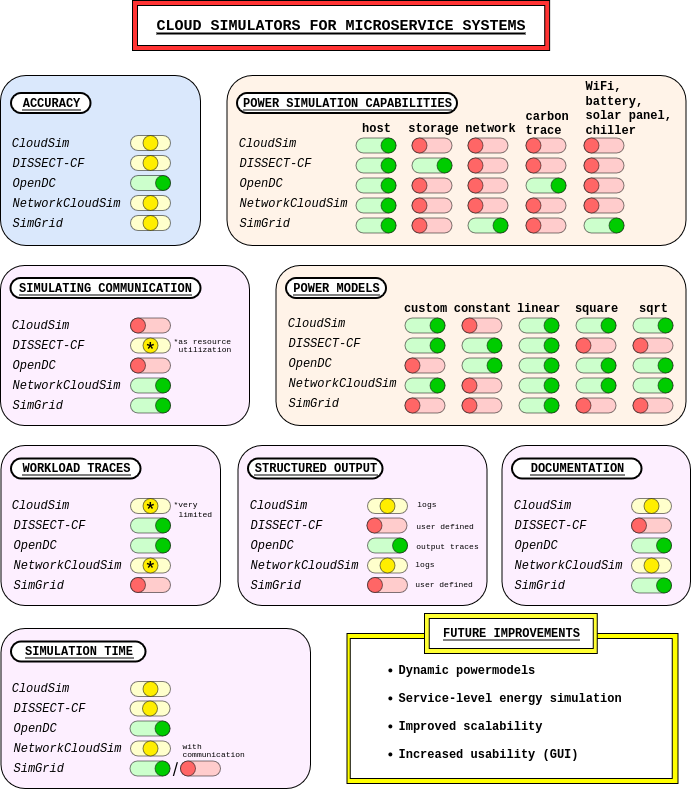
\includegraphics[width=0.85\linewidth]{figures/final.png}
    \caption{Graphic giving an overview of the discussed simulators' properties.}
    % \Description{Graphic giving an overview of the discussed simulators' properties.}
    \label{fig:final}
\end{figure*}

\bibliographystyle{elsarticle-num}
\bibliography{references}

\onecolumn
\newpage
%\appendix
\section{Simulator Selection}
\begin{table*}[ht]
\caption{The 13 selected cloud simulator review papers used to extract cloud simulators from.}
\label{tab:papersAppendix}
\begin{tabularx}{\textwidth}{l>{\raggedright\arraybackslash}X>{\raggedright\arraybackslash}X>{\raggedright\arraybackslash}Xr}
\textbf{Id} &
  \textbf{Title} &
  \textbf{Authors} &
  \textbf{Venue} &
  \textbf{Year} \\ \hline
P1 &
  Cloud computing simulators: A comprehensive review &
  Najme Mansouri, Reyhane Ghafari, Behnam Mohammad, Hasani Zade, &
  Simulation Modelling Practice and Theory &
  2020 \\ \hline
P2 &
  Cloud computing simulators: A detailed survey and future direction &
  Arif Ahmed, Abadhan Saumya Sabyasachi &
  International Advance Computing Conference (IACC) &
  2014 \\ \hline
P3 &
  A Review of Cloud Computing Simulation Platforms and Related Environments &
  James Byrne, Sergej Svorobej, Konstantinos M. Giannoutakis, Dimitrios Tzovaras, P. J. Byrne, Per-Olov Östberg, Anna Gourinovitch, Theo Lynn &
  International Conference on Cloud Computing and Services Science (CLOSER) &
  2017 \\ \hline
P4 &
  Modeling and simulation of cloud computing: A review &
  Wei Zhao, Yong Peng, Feng Xie, Zhonghua Dai &
  Asia Pacific Cloud Computing Congress (APCloudCC) &
  2013 \\ \hline
P5 &
  A Survey on Cloud Computing Simulation and Modeling &
  Ailyas Bambrik &
  SN Computer Science &
  2020 \\ \hline
P6 &
  Simulation tools for cloud computing: A survey and comparative study &
  Fairouz Fakhfakh, Hatem Hadj Kacem, Ahmed Hadj Kacem &
  International Conference on Computer and Information Science (ICIS) &
  2017 \\ \hline
P7 &
  Building a cloud on earth: A study of cloud computing data center simulators &
  Mohamed Abu Sharkh, Ali Kanso, Abdallah Shami, Peter Öhlén &
  Computer Networks &
  2016 \\ \hline
P8 &
  Energy-driven cloud simulation: existing surveys, simulation supports, impacts and challenges &
  Azlan Ismail &
  Cluster Computing &
  2020 \\ \hline
P9 &
  Cloud Computing Simulators: A Review &
  Yousef Sanjalawe, Salam Al-E’mari &
  International Arab Conference on Information Technology (ACIT) &
  2023 \\ \hline
P10 &
  A Comprehensive Survey on Cloud Computing Simulators &
  Oladosu Oyebisi Oladimeji, Dasola Oyeyiola, Olayanju Oladineji, Pelumi Oyeyiola &
  Scientific Journal of Informatics &
  2021 \\ \hline
P11 &
  Evaluation of cloud simulators for energy-related applications &
  Vincenzo Emanuele Martone, Michele Mastroianni, Francesco Palmieri &
  International Conference on Innovation and Intelligence for Informatics, Computing, and Technologies (3ICT) &
  2023 \\ \hline
P12 &
  Cloud Computing and Simulation Paradigms: A Technical Exploration and Analysis &
  Divya Kapil, Varsha Mittal, Atika Gupta &
  International Conference on Computing Communication and Networking Technologies (ICCCNT) &
  2024 \\ \hline
P13 &
  A Systematic Parameter Analysis of Cloud Simulation Tools in Cloud Computing Environments &
  Muhammad Asim Shahid, Muhammad Mansoor Alam, Mazliham Mohd Su’ud &
  Applied Sciences &
  2023 \\
\end{tabularx}
\end{table*}

\newpage

\begin{longtable}[t]{llllllll}
    \caption{The 67 extracted simulators from which the 5 simulators discussed in this study were selected. The simulators suggested by the research practitioner are labelled as having been extracted from \textit{Manual}.}
    \label{tab:allSimulatorsAppendix} 
    \endfirsthead
    \\
    \caption{Continued}\\
    \textbf{\begin{tabular}[b]{@{}l@{}}Name\end{tabular}} &
    \textbf{\begin{tabular}[b]{@{}l@{}}Based on\end{tabular}} &
    \textbf{\begin{tabular}[b]{@{}l@{}}First\\ Published\end{tabular}} &
    \textbf{\begin{tabular}[b]{@{}l@{}}Last\\ Update\end{tabular}} &
    \textbf{Extracted from} &
    \textbf{\begin{tabular}[b]{@{}l@{}}Code\\ available\end{tabular}} &
    \textbf{\begin{tabular}[b]{@{}l@{}}Energy\\ simulation\end{tabular}} \\
    \hline
    \endhead
    %
    \textit{OpenDC} & - & 2021 & 2025 & Manual & \yes & \yes \\ \arrayrulecolor{lightgray} \hline 
    \textit{NetworkCloudSim} & CloudSim & 2011 & 2025 & \begin{tabular}[t]{@{}l@{}}P1, P2, P3, P4,\\ P5, P6, P7, P10,\\ Manual\end{tabular} & \yes & \yes \\ \hline 
    \textit{CloudSim} & GridSim & 2009 & 2025 & \begin{tabular}[t]{@{}l@{}}P1, P2, P3, P4,\\ P5, P6, P7, P8,\\ P9, P10, P11, P12,\\ P13, Manual\end{tabular} & \yes & \yes \\ \hline 
    \textit{SimGrid} & - & 2008 & 2025 & P3, P12 & \yes & \yes \\ \hline 
    \textit{IoTSim-Stream} & CloudSim & 2019 & 2024 & P5 & \yes & \yes \\ \hline 
    \textit{Ds-Sim} & - & 2019 & 2024 & P10 & \yes & \no \\ \hline 
    \textit{CloudSim Plus} & CloudSim & 2017 & 2024 & P13, Manual & \yes & \yes \\ \hline 
    \textit{OCT} \\ \textit{(Open Cloud Testbed)} & - & 2009 & 2024 & P4 & \yes & \no \\ \hline 
    \textit{WCSim} & - & 2023 & \multicolumn{1}{l}{-} & Manual & \no & \no \\ \hline 
    \textit{DISSECT-CF} & - & 2015 & 2023 & \begin{tabular}[t]{@{}l@{}}P1, P3, P5, P8,\\ P11, P12\end{tabular} & \yes & \yes \\ \hline 
    \textit{SCORE} & {\begin{tabular}[b]{@{}l@{}}Google Omega\\simulator\end{tabular}} & 2018 & 2022 & P1 & \yes & \yes \\ \hline 
    \textit{GPUCloudSim} & CloudSim & 2018 & 2022 & P5 & \yes & \yes \\ \hline 
    \textit{DCworms} & GSSIM & 2013 & 2022 & \begin{tabular}[t]{@{}l@{}}P5\\ P8\end{tabular} & \yes & \yes \\ \hline 
    \textit{iFogSim} & iCloudSim & 2017 & 2021 & P3, P5, P12 & \yes & \yes \\ \hline 
    \textit{BigDataSDNSim} & \begin{tabular}[t]{@{}l@{}}CloudSimSDN,\\ IoTSim\end{tabular} & 2020 & 2020 & P5 & \yes & \yes \\ \hline 
    \textit{CloudSimSDN} & CloudSim & 2015 & 2020 & P3, P5, P12 & \yes & \yes \\ \hline 
    \textit{VMPlaces} & - & 2015 & 2020 & P5 & \yes & \no \\ \hline 
    \textit{DFaaSCloud} & CloudSim & 2019 & 2019 & P5 & \yes & \yes \\ \hline 
    \textit{CactoSim} & \begin{tabular}[t]{@{}l@{}}Palladio,\\ SimuLizar\end{tabular} & 2014 & 2019 & P3 & \yes & \yes \\ \hline 
    \textit{GAME-SCORE} & SCORE & 2018 & 2019 & P1, P11 & \yes & \yes \\ \hline 
    \textit{NutShell} & NS3 & 2019 & \multicolumn{1}{l}{-} & P5 & \no & \no \\ \hline 
    \textit{CloudSimDisk} & CloudSim & 2015 & 2018 & \begin{tabular}[t]{@{}l@{}}P3\\ P5\end{tabular} & \yes & \yes \\ \hline 
    \textit{FederatedCloudSim} & CloudSim & 2014 & 2017 & P1 & \yes & \yes \\ \hline 
    \textit{CloudReports} & CloudSim & 2014 & 2017 & P1, P3, P5, P6 & \yes & \yes \\ \hline 
    \textit{ElasticSim} & CloudSim & 2017 & 2016 & P1, P6 & \yes & \yes \\ \hline 
    \textit{CM Cloud} & CloudSim & 2016 & 2016 & P1 & \yes & \yes \\ \hline 
    \textit{CloudAuction} & CloudSim & 2015 & 2016 & P12 & \yes & \yes \\ \hline 
    \textit{Bazaar-Extension} & CloudSim & 2016 & \multicolumn{1}{l}{-} & P3, P5 & \no & \yes \\ \hline 
    \textit{ATAC4Cloud} & CloudSim & 2016 & \multicolumn{1}{l}{-} & P5 & \no & \yes \\ \hline 
    \textit{CloudSimEx} & CloudSim & 2012 & 2015 & P12 & \yes & \yes \\ \hline 
    \textit{CEPSim} & CloudSim & 2015 & 2015 & P1, P3, P5, P6 & \yes & \yes \\ \hline 
    \textit{DesktopCloudSim} & CloudSim & 2015 & 2015 & P5 & \yes & \yes \\ \hline 
    \textit{DynamicCloudSim} & CloudSim & 2014 & 2015 & P1, P5 & \yes & \yes \\ \hline 
    \textit{GloudSim} & - & 2014 & 2015 & P5 & \yes & \no \\ \hline 
    \textit{CloudSched} & - & 2013 & 2015 & \begin{tabular}[t]{@{}l@{}}P1, P3, P5, P6,\\ P8\end{tabular} & \yes & \yes \\ \hline 
    \textit{WorkflowSim} & CloudSim & 2012 & 2015 & P1, P3, P5, P6 & \yes & \yes \\ \hline 
    \textit{iCanCloud} & SIMCAN & 2012 & 2015 & \begin{tabular}[t]{@{}l@{}}P1, P2, P3, P4,\\ P5, P6, P7, P9, \\Manual\end{tabular} & \yes & \yes \\ \hline 
    \textit{SimGrid VM} & - & 2015 & \multicolumn{1}{l}{-} & P5 & \no & \no \\ \hline 
    \textit{CloudExp} & CloudSim & 2014 & 2014 & P1, P3, P5, P6 & \yes & \yes \\ \hline 
    \textit{CloudNetSim++} & OMNeT++ & 2014 & 2014 & P1, P3, P8 & \yes & \yes \\ \hline 
    \textit{Cloud2Sim} & \begin{tabular}[t]{@{}l@{}}CloudSim,\\ Hazelcast,\\ Infinispan\end{tabular} & 2014 & 2014 & P3, P5 & \yes & \yes \\ \hline 
    \textit{CloudSimScale} & CloudSim & 2014 & 2014 & P5 & \yes & \yes \\ \hline 
    \textit{TeachCloud} & CloudSim & 2013 & 2014 & P1, P3, P6, P7 & \yes & \yes \\ \hline 
    \textit{CRest} & - & 2013 & 2014 & P5 & \yes & \yes \\ \hline 
    \textit{DCSim} & - & 2012 & 2014 & \begin{tabular}[t]{@{}l@{}}P2, P3, P4, P5,\\ P6, P8, P10\end{tabular} & \yes & \yes \\ \hline 
    \textit{secCloudSim} & iCanCloud & 2014 & \multicolumn{1}{l}{-} & P1, P6 & \no & \no \\ \hline 
    \textit{GreenCloud} & NS2 & 2010 & 2013 & \begin{tabular}[t]{@{}l@{}}P1, P2, P3, P4,\\ P6, P7, P8, P9,\\ P10, P11, P12,\\ Manual\end{tabular} & \yes & \yes \\ \hline 
    \textit{CloudNetSim} & - & 2013 & \multicolumn{1}{l}{-} & P1 & \no & \no \\ \hline 
    \textit{SimIC} & - & 2013 & \multicolumn{1}{l}{-} & \begin{tabular}[t]{@{}l@{}}P1, P2, P5, P6,\\ P10\end{tabular} & \no & \yes \\ \hline 
    \textit{E-mc2} & iCanCloud & 2013 & \multicolumn{1}{l}{-} & P5, P8 & \no & \yes \\ \hline 
    \textit{SGCB} \\ \textit{+(SimGrid Cloud Broker)} & SimGrid & 2013 & \multicolumn{1}{l}{-} & P5 & \no & \no \\ \hline 
    \textit{DartCSim+} & CloudSim & 2013 & \multicolumn{1}{l}{-} & P1 & \no & \yes \\ \hline 
    \textit{FTCloudSim} & CloudSim & 2013 & \multicolumn{1}{l}{-} & P1, P6, P9 & \no & \yes \\ \hline 
    \textit{EMUSim} & \begin{tabular}[t]{@{}l@{}}AEF, CloudSim\end{tabular} & 2012 & 2012 & \begin{tabular}[t]{@{}l@{}}P1, P2, P3, P4,\\ P5, P6, P9\end{tabular} & \yes & \yes \\ \hline 
    \textit{BigHouse} & - & 2012 & 2012 & P7, P8 & \yes & \yes \\ \hline 
    \textit{SPECI} & - & 2009 & 2012 & \begin{tabular}[t]{@{}l@{}}P1, P3, P4, P5,\\ P6, P7\end{tabular} & \no & \no \\ \hline 
    \textit{MR-CloudSim} & CloudSim & 2012 & \multicolumn{1}{l}{-} & P1, P2, P3, P6 & \no & \yes \\ \hline 
    \textit{UCloud} & CloudSim & 2012 & \multicolumn{1}{l}{-} & P1, P3 & \no & \yes \\ \hline 
    \textit{SmartSim} & - & 2012 & \multicolumn{1}{l}{-} & P2, P5 & \no & \yes \\ \hline 
    \textit{CDOSim} & CloudSim & 2012 & \multicolumn{1}{l}{-} & P1, P2, P3, P7 & \no & \yes \\ \hline 
    \textit{DartCSim} & CloudSim & 2012 & \multicolumn{1}{l}{-} & P1, P3, P6 & \no & \yes \\ \hline 
    \textit{CloudAnalyst} & CloudSim & 2009 & 2010 & \begin{tabular}[t]{@{}l@{}}P1, P2, P3, P4,\\ P5, P6, P7, P9,\\ P10, P12, P13,\\ Manual\end{tabular} & \yes & \yes \\ \hline 
    \textit{GDCSim} & - & 2011 & \multicolumn{1}{l}{-} & \begin{tabular}[t]{@{}l@{}}P1, P3, P5, P7,\\ P8, P11\end{tabular} & \no & \yes \\ \hline 
    \textit{GroudSim} & - & 2011 & \multicolumn{1}{l}{-} & \begin{tabular}[t]{@{}l@{}}P1, P2, P3, P4,\\ P5, P6, P7, P10, \\Manual\end{tabular} & \no & \no \\ \hline 
    \textit{MDCSim} & CSIM & 2009 & \multicolumn{1}{l}{-} & \begin{tabular}[t]{@{}l@{}}P1, P2, P3, P5,\\ P6, P7, P8, P10\end{tabular} & \no & \yes \\ \hline 
    \textit{Open Cirrus} & - & 2009 & \multicolumn{1}{l}{-} & P4 & \no & \no \\ \hline 
    \textit{DGSim} & - & 2008 & \multicolumn{1}{l}{-} & Manual & \no & \no
\end{longtable}

\newpage
\section{Simulator Output Screenshots}
\subsection{\textit{CloudSim} and \textit{NetworkCloudSim}}

\begin{figure}[h]
    \centering
    \includegraphics[width=0.5\linewidth]{vu-cs-research-thesis/figures/sc-cloudsim.png}
    \caption{Screenshot of the end of terminal output of an example \textit{CloudSim} or \textit{NetworkCloudSim} simulation.}
    % \Description{Screenshot of the end of terminal output of an example \textit{CloudSim} or \textit{NetworkCloudSim} simulation.}
    \label{fig:scCloudsim}
\end{figure}

\subsection{\textit{DISSECT-CF}}
\begin{figure}[h]
    \centering
    \includegraphics[width=0.8\linewidth]{vu-cs-research-thesis/figures/sc-dissectcf.png}
    \caption{Screenshot of terminal output of an example \textit{DISSECT-CF} simulation.}
    % \Description{Screenshot of terminal output of an example \textit{DISSECT-CF} simulation.}
    \label{fig:scDissectCF}
\end{figure}

\subsection{\textit{OpenDC}}
\begin{figure}[h]
    \centering
    \includegraphics[width=0.45\linewidth]{vu-cs-research-thesis/figures/sc-opendc.png}
    \caption{Screenshot of the end of terminal output of an example \textit{OpenDC} simulation.}
    % \Description{Screenshot of the end of terminal output of an example \textit{OpenDC} simulation.}
    \label{fig:scOpenDC}
\end{figure}

\newpage
\subsection{\textit{SimGrid}}
\begin{figure}[h]
    \centering
    \includegraphics[width=0.55\linewidth]{vu-cs-research-thesis/figures/sc-simgrid.png}
    \caption{Screenshot of the end of terminal output of an example \textit{SimGrid} simulation.}
    % \Description{Screenshot of the end of terminal output of an example \textit{SimGrid} simulation.}
    \label{fig:scSimGrid}
\end{figure}

\end{document}


%%% Local Variables:
%%% mode: latex
%%% TeX-master: t
%%% End:
